
\documentclass[11pt]{report}
\usepackage{makeidx}
\usepackage{url}
\usepackage{a4wide}
\usepackage{longtable}
\usepackage{color}
\usepackage{alltt,xspace}
\usepackage[colorlinks]{hyperref}
\usepackage{subfigure,graphicx,epsfig,epsf,amsmath,amsfonts,float}
\usepackage{fancyheadings}
\usepackage{datetime}
\usepackage{relsize}
\usepackage{etoolbox} %% support for conditional compilation


\parskip5pt
\parindent0pt
\sloppy 
%%\newcommand{\FLORA}{{\mbox{\sc ${\cal F}${lora}\rm\emph{-2}}}\xspace}
\newcommand{\FLORA}{{\mbox{\smaller{\sc ${\cal F}${lora}\rm\emph{-2}}}}\xspace}
\newcommand{\ERGO}{\mbox{\smaller{\ensuremath{\cal{E}}\smaller{{\sc{RGO}}}}}\xspace}
\newcommand{\ERGOAI}{\mbox{\smaller{\ensuremath{\cal{E}}\smaller{{\sc{RGO}}}\ensuremath{\cal{AI}}}}\xspace}
\newcommand{\ERGOLITE}{\mbox{\smaller{\ensuremath{\cal{E}}\smaller{{\sc{RGO}\ensuremath{^{Lite}}}}}}\xspace}
%%\newcommand{\ERGO}{\ensuremath{\cal{E}\mbox{\smaller{\sc{RGO}}}}\xspace}
%%\newcommand{\ERGO}{\ensuremath{\cal{E}\mbox{\smaller{{\sc{RGO}}}}}\xspace}
%%\newcommand{\ERGOAI}{\ensuremath{\cal{E}\mbox{\smaller{{\sc{RGO}}}}\!\cal{AI}}\xspace}
%%\newcommand{\ERGOLITE}{\ensuremath{\cal{E}\mbox{\smaller{\sc{RGO}\ensuremath{^{Lite}}}}}\xspace}
\newcommand{\FLSYSTEM}{\FLORA}
\newcommand{\FLRCFILE}{\texttt{FLORA\_RC\_FILE}\xspace}
\newcommand{\FLABORT}{FLORA\_ABORT}
\newcommand{\flabort}{'\_\$flora\_abort'}
\newcommand{\FLUSERABORT}{FLORA\_USER\_ABORT}
\newcommand{\FLUNDEFEXCEPTION}{FLORA\_UNDEFINED\_EXCEPTION}
\newcommand{\FLDBEXCEPTION}{FLORA\_DB\_EXCEPTION}
\newcommand{\flundefexception}{'\_\$flora\_undefined'}
\newcommand{\fldbexception}{'\_\$flora\_db\_error'}
\newcommand{\FLPREFIX}{\_\$\_\$\_flora}

\newcommand{\FLSHELL}{flora\_shell}
\newcommand{\FLBOOTSTRAP}{bootstrap\_flora}
\newcommand{\FLQUERYCMD}{flora\_query}

\newcommand{\FLORAMODE}{flora-mode}
\newcommand{\FLORAFILE}{flora.elc}
\newcommand{\FLORAFILEBASE}{flora}

\newcommand{\ENGINENAME}{flora2}
\newcommand{\ENGINENAMEALT}{flora2}
\newcommand{\ENGINERUN}{runflora}

\newcommand{\prompt}{flora2 ?- }
\newcommand{\errorsystem}{Flora-2}
\newcommand{\floraname}{Flora-2}
\newcommand{\flrext}{flr}
\newcommand{\flrextemacs}{"\bs{}\bs{}.flr\$"}

\IfFileExists{../ergoisms/ergo.switch}{\input{./ergoisms/definitions}}{\newcommand{\isfloraman}{yes}}

\newcommand{\fl}{F-logic }

\newcommand{\fd}{{\mbox{\tt \,->\,}}}                   % scalar
\newcommand{\mvd}{{\mbox{\tt \,->\,}}}  % multivalued
\newcommand{\Fd}{{\mbox{\tt \,=>\,}}}                      % scalar signature
\newcommand{\Mvd}{{\mbox{\tt \,=>\,}}}  % multivalued signature
\newcommand{\thismodule}{{\tt \_@}\xspace}
\newcommand{\bs}{{\ensuremath\backslash}}

\def\Protege{Prot\'{e}g\'{e} }
\def\NoProtege{Prot\'{e}g\'{e}}

\ifdef{\isfloraman}{
  \title{\bf A Guide to \FLSYSTEM Packages
    \vspace{0.7cm}\\
    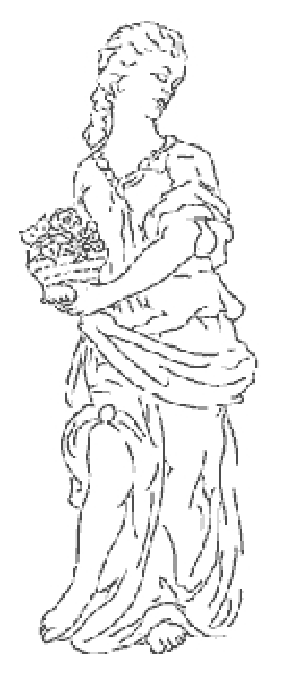
\includegraphics[width=1in]{floralogo} 
    \vspace{3mm}\\
    {\Large Version 2.0}
    \\
    {\large (Pyrus nivalis)}
    \vspace{0.9in}
\begin{center}
  \large\textnormal{
  \monthname ~\the\year
  }
\end{center}
  }
}
{
  \input{./ergoisms/pkg-title}
}

\date{}

\makeindex 
\begin{document}

\pagenumbering{Alph}
\maketitle


\thispagestyle{empty}
\bibliographystyle{plain}
%%\newpage
%%\thispagestyle{empty}

\pagenumbering{roman}
\setcounter{page}{1}
\tableofcontents
\newpage        % Just to avoid a silly LaTeX bug with \pagenumbering
  
\pagenumbering{arabic}



\chapter[JAVA-to-\FLSYSTEM Interfaces]
{JAVA-to-\FLSYSTEM Interfaces\\
  {\Large by Aditi Pandit and Michael Kifer}}


This chapter documents the API for accessing \FLSYSTEM from Java
programs.  The API has two versions: a \emph{low-level API} (used most
commonly), which
enables Java programs to send arbitrary queries to \FLSYSTEM and
get results, and an \emph{experimental}
\emph{high-level API}, which is more limited and requires some setup,
but can simplify a number of tasks in interfacing the two systems. The high-level API establishes a
correspondence between Java classes and \FLSYSTEM classes, which
enables manipulation of \FLSYSTEM classes by executing appropriate
methods on the corresponding Java classes. Both interfaces rely on
the Java-XSB interface, called \emph{Interprolog} \cite{Calejo2004}, developed by
\url{http://interprolog.com/}.

The API assumes that a Java program is started first and then it invokes
XSB/\FLSYSTEM as a subprocess. The XSB/\FLSYSTEM side is passive: it only
responds to the queries sent by the Java side.
Queries can be anything that is accepted at the \FLSYSTEM
shell prompt: queries, insert/delete commands, control switches, etc., are
all fine.
One thing to remember is that the backslash is used in Java
as an escape symbol and in \FLSYSTEM as a prefix of the builtin operators
and commands. Therefore, each backslash must be escaped with another
backslash. That is, instead of a query like "\texttt{p(?X) \bs{}and q(?X).}"
the API requires "\texttt{p(?X) \bs{}\bs{}and q(?X)}.".

\paragraph{The \texttt{FloraObject} object.}
While reading this document one will notice that the class
\texttt{FloraObject} is used in many cases. This class consists of
Java objects that
encapsulate  \FLSYSTEM objects. These Java objects
are mostly used internally.
From the end user's point of view, the only method of interest in this
class is
\texttt{toString()}. 


\section{The Low-level Interface} \label{sec-java-lowlevel}
 The low-level API enables Java programs to send arbitrary queries
to \FLSYSTEM and get results. 
It is assumed that the following two Java properties
are set either as part of the java command (e.g.,  \texttt{java
  ... -DPROLOGDIR=some-dir ...}) or inside the Java application itself, e.g.,
%% 
\begin{verbatim}
System.setProperty("PROLOGDIR","C:\\JSmith\\XSB\\config\\x64-pc-windows\\bin");
\end{verbatim}
%%
Please remember that Windows uses backslash as a file separator, and inside a
Java program these backslashes must be doubled, as shown above.

The two aforementioned properties are:
\begin{description}
\item[\texttt{PROLOGDIR}:] 
This variable points to the folder
containing the XSB executable (binary, not the command script).
\\
To get the right value for your installation, start
\FLSYSTEM and execute this at the prompt:
%% 
\begin{verbatim}
system{bindir = ?D}.
\end{verbatim}
%% 
The result will be returned in the variable \texttt{?D}. 

\item[{\tt FLORADIR}:]
\label{page-floradir}
  This variable must point to the folder
containing the \FLSYSTEM installation.
\\
To get the right value for your installation, start
\FLSYSTEM and execute this at the prompt:
%% 
\begin{verbatim}
system{installdir = ?D}.
\end{verbatim}
%% 
Again, the result will be returned in the variable \texttt{?D}. 
\end{description}
  %%

\bigskip

In order to be able to access \FLSYSTEM, the Java program must first establish
a session for a running instance of \FLSYSTEM. Multiple sessions can be active
at the same time. The knowledge bases in the different running instances
are completely independent. Sessions are instances of
the class {\tt net.sf.flora2.API.FloraSession}. This class provides methods
for opening/closing sessions and loading \FLSYSTEM knowledge bases
(which are also used in the high-level
interface). In addition, a session provides 
methods for executing arbitrary \FLSYSTEM queries. The following is the complete
list of the methods that are available in that class.
All these are \emph{public}
\emph{instance} methods  and the word ``public'' is therefore omitted.
%%
\begin{itemize}
\item
\begin{verbatim}
FloraSession()
\end{verbatim}
  This constructor creates a connection to an instance of \FLSYSTEM.
  Use it like this:
  %% 
\begin{verbatim}
    FloraSession session = new FloraSession();
\end{verbatim}
  %% 
  All the methods below are executed on \texttt{FloraSession}-objects
  produced in this way. 
\item {\tt close()} \\
  This method must be called to terminate a \FLSYSTEM session. Note that this does
  not terminate the Java program that initiated the session:
  to exit the Java program that talks to \FLSYSTEM, one needs to execute
  the statement
  %%
\begin{verbatim}
 System.exit();  
\end{verbatim}
  %%
  Note that just returning from the {\tt main} method is not enough. 

\item
\begin{verbatim}
Iterator<FloraObject> executeQuery(String query)
\end{verbatim}
    This method executes the \FLSYSTEM query given by the
parameter {\tt query}.
The query must be terminated with a period, exactly as it would be typed
in the \FLSYSTEM shell.
It is used to execute \FLSYSTEM queries that
do not require variable bindings to be returned back to Java \emph{or} queries that
have only
a single variable to be returned. Each binding is represented as
an instance of the class {\tt net.sf.flora2.API.FloraSession}.
The examples below illustrate how to process the results returned by this
method.

\item
\begin{verbatim}
Iterator<HashMap<String,FloraObject>> executeQuery(String query,Vector vars)
\end{verbatim}
  This method executes the \FLSYSTEM query given by the first argument.
The query must be terminated with a period, as if it were typed
in the \FLSYSTEM shell.
 The Vector {\tt vars} (of strings) specifies the names of all the variables
  in the query for which bindings need to be returned. These variables are
  added to the vector using the method {\tt add} before calling
  {\tt executeQuery}. For instance, {\tt vars.add("?X")}.  
  
  This version of {\tt executeQuery} returns an iterator over all bindings
  returned by the \FLSYSTEM query.  Each binding is represented by a {\tt
    HashMap<String,FloraObject>} 
  object which can be used to obtain the value of each variable in the
  query (using the {\tt get()} method). The value of each variable returned
  is an instance of {\tt net.sf.flora2.API.FloraObject}.

  The examples below show how to handle the results returned by this method.

\item \texttt{boolean executeCommand(String command)} \\
  This is a simplified way of executing \FLSYSTEM queries that \emph{do not need}
  to return any results, i.e., when the user wants to know if the query is
  true or false for \emph{some} bindings of command's arguments (if there
  are any), but not the actual bindings.
  There are also differences (compared to \texttt{executeQuery()})
  in the way this command handles exceptions, as
  explained in the next section.
  As before, the command must be terminated with a period.

\item
\begin{verbatim}
boolean loadFile(String fileName,String moduleName)
\end{verbatim}
  This method loads the \FLSYSTEM program, specified by the parameter {\tt
    fileName} into the \FLSYSTEM module specified in {\tt moduleName}.
  If errors occur during loading, \texttt{loadFile()} returns \texttt{false}.  
\item
\begin{verbatim}
boolean compileFile(String fileName,String moduleName)
\end{verbatim}
  This method compiles (but does not load)
  the \FLSYSTEM program, specified by the parameter {\tt
    fileName} for the \FLSYSTEM module specified in {\tt moduleName}.
  If errors occur during compilation, \texttt{compileFile()} returns \texttt{false}.  
\item
\begin{verbatim}
boolean addFile(String fileName,String moduleName)
\end{verbatim}
  This method adds the \FLSYSTEM program, specified by the parameter {\tt
    fileName} to an existing \FLSYSTEM module specified in {\tt moduleName}.
  If errors occur during addition, \texttt{addFile()} returns \texttt{false}.  
\item
\begin{verbatim}
boolean compileaddFile(String fileName,String moduleName)
\end{verbatim}
  This method compiles the \FLSYSTEM program, specified by the parameter {\tt
    fileName} for addition to the \FLSYSTEM module specified in {\tt moduleName}.
  If errors occur during compilation, \texttt{compileaddFile()} returns \texttt{false}.  
\end{itemize}

The code snippet below illustrates the low-level API.

\paragraph{Step 1: Writing \FLSYSTEM programs to be called by Java.}
  Let us assume that we have a file, called  {\tt flogic\_basics.flr},
  which contains the following information:
\begin{quote}
\begin{verbatim}
person :: object.
dangerous_hobby :: object.
john:employee.
employee::person.

bob:person.
tim:person.
betty:employee.

person[|age=>integer,
       kids=>person,
       salary(year)=>value,
       hobbies=>hobby,
       believes_in=>something,
       instances => person
|].

mary:employee[
    age->29,
    kids -> {tim,leo,betty},
    salary(1998) -> a_lot
].

tim[hobbies -> {stamps, snowboard}].
betty[hobbies->{fishing,diving}].

snowboard:dangerous_hobby.
diving:dangerous_hobby.

?_X[self-> ?_X].

person[|believes_in -> {something, something_else}|].
\end{verbatim}
\end{quote}

\paragraph{Step 2:  Writing a JAVA application to interface with \FLSYSTEM.}
 The following code loads a \FLSYSTEM program from a file and then passes
 queries to the knowledge base.

\begin{verbatim}
import java.util.*;
import net.sf.flora2.API.*;
import net.sf.flora2.API.util.*;

public class flogicbasicsExample {

    public static void main(String[] args) {
        // create a new session for a running instance of the engine
        FloraSession session = new FloraSession();
        System.out.println("Engine session started");

        // Assume that Java was called with -DINPUT_FILE=the-file-name
        String fileName = System.getProperty("INPUT_FILE");
        if(fileName == null || fileName.trim().length() == 0) {
            System.out.println("Invalid path to example file!");
            System.exit(0);

        }
        // load the program into module basic_mod
        if (session.loadFile(fileName,"basic_mod"))
            System.out.println("Example loaded successfully!");
        else
            System.out.println("Error loading the example!");

        /* Running queries from flogic_basics.flr */

        /* Query for persons */
        String command = "?X:person@basic_mod.";
        System.out.println("Query:"+command);
        Iterator<FloraObject> personObjs = session.executeQuery(command);

        /* Printing out the person names and information about their kids */
        while (personObjs.hasNext()) {
            FloraObject personObj = personObjs.next();
            System.out.println("Person name:"+personObj);
        }

        command = "person[instances -> ?X]@basic_mod.";
        System.out.println("Query:"+command);
        personObjs = session.executeQuery(command);

        /* Printing out the person names  */
        while (personObjs.hasNext()) {
            Object personObj = personObjs.next();
            System.out.println("Person Id: "+personObj);
        }

        /* Example of executeQuery with two arguments */
        Vector<String> vars = new Vector<String>();
        vars.add("?X");
        vars.add("?Y");

        Iterator<HashMap<String,FloraObject>> allmatches =
            session.executeQuery("?X[believes_in -> ?Y]@basic_mod.",vars);
        System.out.println("Query:?X[believes_in -> ?Y]@basic_mod.");
        while(allmatches.hasNext()) {
            HashMap<String,FloraObject> firstmatch = allmatches.next();
            Object Xobj = firstmatch.get("?X");
            Object Yobj = firstmatch.get("?Y");
            System.out.println(Xobj+" believes in: "+?Yobj);
        }
        // quit the system
        session.close();
        System.exit(0);
    }
}
\end{verbatim}

 For the information on how to invoke the above Java class in the context
 of the Java-\FLSYSTEM API,
 please see Section~\ref{sec-executing-apps}.

\section{Debugging \FLSYSTEM Statements Used in a Java Program}

\subsection{Logging}

It often happens that an \FLSYSTEM query or a file used from within a Java
Program has an error and \texttt{executeQuery()} returns an error message
saying that there is a ``problem'' with a \FLSYSTEM statement.
The Java part does not know what the problem is but it can be told to show
the output of the \FLSYSTEM statements on the console. This can be done by
executing the statement
%% 
\begin{verbatim}
    FloraSession.showOutput();
\end{verbatim}
%% 
This will stream all warnings, errors, and just normal output from
\FLSYSTEM to the console.
When no longer needed, this mode can be turned off like this:
%% 
\begin{verbatim}
    FloraSession.hideOutput();
\end{verbatim}
%% 
The \texttt{FloraSession.showOutput();} statement can be executed at any
point in the program, but preferably after calling \texttt{FloraSession()},
to avoid irrelevant output.

Here is an example of what you might see:
%% 
\begin{verbatim}
My command 2 has succeeded

yes

Loading file test.ergo:

yes

++Error[Ergo]> [test.ergo] <Composer> near line(2)/char(3) `b' unexpected operand:
 ',', '.', or some other operator may be missing just before the indicated location

++1 error

++compilation aborted
\end{verbatim}
%% 
Here the output from \FLSYSTEM starts with normal output from, say,
\texttt{writeln(...)@\bs{}io} commands and ends with a compilation error
encountered while compiling the file \texttt{test.ergo}.  
(The above is output from \ERGO; in \FLORA it will be similar.)

Two other useful calls are
%% 
\begin{verbatim}
    FloraSession.enableLogging();
    FloraSession.disableLogging();
\end{verbatim}
%%
Executing \texttt{FloraSession.enableLogging();} will cause the Java API to
record all major events such as starting a session, ending it, loading or
adding a \FLSYSTEM file, and execution of every query. It does not report
query answers, however. Logging can be enabled or disabled anywhere in the
program, but, of course, the log messages will start to appear only after
the enabling command is executed and will cease to appear after
\texttt{disableLogging()} is executed. 

\subsection{Catching Exceptions, Checking Errors and Warnings}

Logging allows one to find errors and warnings in an \FLSYSTEM
subprocess of a Java program by checking the output produced by the session.
However, often one needs to be able to do this \emph{programmatically}  and
this can be done as follows.

\paragraph{Exceptions.} First, if a running \FLSYSTEM query invoked via
\texttt{executeQuery()}
issues a
run-time error, a Java \texttt{FlrException} is thrown, and this can be
caught by the parent Java program.
An exception is also thrown if the query passed to \texttt{executeQuery()}
has a syntax error.\footnote{
  If the query statement itself has no syntax error but it loads a file
  that has a syntax error then \emph{no} exception is thrown. Read on to
  see how to identify this situation programmatically.
}
%% 
Note that \FLSYSTEM statements invoked via 
the other methods (\texttt{executeCommand()},
\texttt{loadFile()}, etc.) do \emph{not} throw  exceptions and errors that
occur during the execution of those statements can be detected only through
the mechanism of \texttt{hasErrors()} described below. 
However, \texttt{executeCommand()}, \texttt{loadFile()},
\texttt{addFile()}, etc., may throw exceptions for other reasons, such as  
a wrong module in \texttt{loadFule()}, etc. 

\paragraph{Detecting syntax errors and warnings.}
Errors and warnings produced
by the \FLSYSTEM compiler do \emph{not} result in exceptions, so they
cannot be caught via Java's try-catch mechanism. To detect if a previous
\texttt{executeQuery()},  \texttt{executeCommand()}, \texttt{loadFile()},
or similar API command produced a warning or an error, use the following
\emph{public} \emph{instance}  methods in class \texttt{FloraSession}:
%% 
\begin{itemize}
\item  \texttt{boolean hasErrors()} --- executing
  \texttt{session.hasErrors()}, where session is a variable holding
  a \texttt{FloraSession}
  object created earlier,
  will tell if a previous \texttt{executeQuery()} or other such
  command (executed on the same \texttt{FloraSession} object)
  has produced an error. This also includes runtime errors, like
  \texttt{FlrException}'s. 
\item  \texttt{boolean hasWarnings()} --- executing
  \texttt{session.hasWarnings()}, where session is a  variable holding
  a \texttt{FloraSession}
  object, will tell if a previous \texttt{executeQuery()} or other such
  command (executed on the same \texttt{FloraSession} object)
  has produced a warning.
\end{itemize}
%% 




\section{The High-Level Interface (experimental)}

The high-level API operates by creating proxy Java classes for 
\FLSYSTEM classes selected by the user.
This enables the Java program to operate on \FLSYSTEM classes by
executing appropriate methods on the corresponding proxy Java classes.
However, compared to the low-level interface, the high-level one is
somewhat limited.  Both interfaces can be used at the same time, if desired.

\textbf{Note A:}  
Most users appear to opt for the low-level interface and such readers
can skip this section.

\textbf{Note B}: This interface will not work for \FLSYSTEM programs that
use \emph{non-alphanumeric} names for methods and predicates. For instance,
if a program involves statements like \texttt{foo['bar\$\#123'->456]} then
the interface might generate syntactically incorrect Java proxy classes and
errors will be issued during the compilation. 

\bigskip

The use of the high-level API involves a number of steps, as described below.

\paragraph{Stage 1: Writing \FLSYSTEM programs to use with the high-level
  interface.}
We assume the same {\tt flogic\_basics.flr} file as in the previous
example.

\paragraph{Stage 2: Generating Java classes that serve as proxies for \FLSYSTEM classes.}
The \FLSYSTEM side of the Java-to-\FLSYSTEM high level API provides a predicate
to generate Java proxy classes for each \fl class which have a signature
declaration in the \FLSYSTEM knowledge base. A proxy class gets defined so
that it would have methods to manipulate the attributes and methods of the
corresponding \fl class for which signature declarations are available.  If
an \fl class has a declared value-returning attribute {\tt foobar} then the
proxy class will have the following methods. Each method name has the form
\emph{action}$S_1S_2S_3$\_{\tt foobar}, where \emph{action} is either {\tt
  get}, {\tt set}, or {\tt delete}. The specifier $S_1$ indicates the type
of the method --- {\tt V} for value-returning, {\tt B} for Boolean, and
{\tt P} for procedural. The specifier $S_2$ tells whether the operation
applies to the signature of the method ({\tt S}), e.g., {\tt
  person[foobar=>string]}, or to the actual data ({\tt D}), for example,
{\tt john[foobar->3]}.  Finally, the specifier $S_3$ tells if the operation
applies to the inheritable variant of the method ({\tt I})
or its non-inheritable variant ({\tt N}).
%% 
\begin{enumerate}
\item {\tt public Iterator<FloraObject> getVDI\_foobar()}\\
  {\tt public Iterator<FloraObject> getVDN\_foobar()}
  \\
  {\tt public Iterator<FloraObject> getVSI\_foobar()}\\
  {\tt public Iterator<FloraObject> getVSN\_foobar()}
  \\
  The above methods query the knowledge base and get all answers for the
  attribute {\tt foobar}. They return iterators through which these answers
  can be processed one-by-one. Each object returned by the iterator is of
  type {\tt FloraObject}.  The {\tt getVDN} form queries non-inheritable
  data methods and {\tt getVDI} the inheritable ones. The {\tt getVSI} and
  {\tt getVSN} forms query the signatures of the attribute {\tt foobar}.
\item {\tt public boolean setVDI\_foobar(Vector value)}\\
  {\tt public boolean setVDN\_foobar(Vector value)}
  \\
  {\tt public boolean setVSI\_foobar(Vector value)}\\
  {\tt public boolean setVSN\_foobar(Vector value)}
  \\
  These methods
  add values to the set of values returned by the attribute {\tt foobar}. The
  values must be placed in the vector parameter passed these methods.
  Again, {\tt setVDN} adds data for non-inheritable methods and {\tt setVDI}
  is used for inheritable methods.
  {\tt setVSI} and {\tt setVSN} add types to signatures.  
\item {\tt public boolean setVDI\_foobar(Object value)}\\
  {\tt public boolean setVDN\_foobar(Object value)}
  \\
  {\tt public boolean setVSI\_foobar(Object value)}\\
  {\tt public boolean setVSN\_foobar(Object value)}\\
  These methods provide a simplified interface when only one value needs to
  be added.  It works like the earlier set\_* methods, except that only one
  value given as an argument is added.
\item {\tt public boolean deleteVDI\_foobar(Vector value)}\\
  {\tt public boolean deleteVDN\_foobar(Vector value)}
  \\
  {\tt public boolean deleteVSI\_foobar(Vector value)}\\
  {\tt public boolean deleteVSN\_foobar(Vector value)}
  \\
  Delete a set of values of the attribute {\tt foobar}. The set is
  specified in the vector argument.
\item {\tt public boolean deleteVDI\_foobar(Object value)}\\
  {\tt public boolean deleteVDN\_foobar(Object value)}
  \\
  {\tt public boolean deleteVSI\_foobar(Object value)}\\
  {\tt public boolean deleteVSN\_foobar(Object value)}
  \\
  A simplified interface for the case when only one value needs to be deleted.
\item {\tt public boolean deleteVDI\_foobar()}\\
  {\tt public boolean deleteVDN\_foobar()}
  \\
  {\tt public boolean deleteVSI\_foobar()}\\
  {\tt public boolean deleteVSN\_foobar()}
  \\
  Delete all values for the attribute {\tt foobar}. 
\end{enumerate}
%% 
For \fl methods with arguments, the high-level API provides Java methods as
above, but they take more arguments to accommodate the parameters that \fl
methods take. Let us
assume that the \fl method is called {\tt foobar2} and it takes parameters
{\tt arg1} and {\tt arg2}.  As before the {\tt getVDI\_*}, {\tt setVDI\_*},
etc., forms of the Java methods are for dealing with inheritable \FLSYSTEM
methods and the {\tt getVDN\_*}, {\tt setVDN\_*},
etc., forms are for dealing with non-inheritable \FLSYSTEM methods.

%%
\begin{enumerate}
\item {\tt public Iterator<FloraObject> getVDI\_foobar2(Object arg1, Object arg2)}\\
  {\tt public Iterator<FloraObject> getVDN\_foobar2(Object arg1, Object arg2)}
  \\
  Obtain all values for the \fl method invocation {\tt foobar2(arg1,arg2)}.
\item {\tt public boolean setVDI\_foobar2(Object arg1, Object arg2, Vector value)}\\
  {\tt public boolean setVDN\_foobar2(Object arg1, Object arg2, Vector value)}
  \\
  Add a set of methods specified in the parameter {\tt value} for the method
  invocation {\tt foobar2(arg1,arg2)}. 
\item {\tt public boolean setVDI\_foobar2(Object arg1, Object arg2, Object value)}\\
  {\tt public boolean setVDN\_foobar2(Object arg1, Object arg2, Object value)}
  \\
  A simplified interface when only one value is to be added.
\item {\tt public boolean deleteVDI\_foobar2(Object arg1, Object arg2, Vector value)}\\
  {\tt public boolean deleteVDN\_foobar2(Object arg1, Object arg2, Vector value)}
  \\
  Delete a set of values from {\tt foobar2(arg1,arg2)}. The set is given by
  the vector parameter {\tt value}. 
\item {\tt public boolean deleteVDI\_foobar2(Object arg1, Object arg2, Object value)}\\
  {\tt public boolean deleteVDN\_foobar2(Object arg1, Object arg2, Object value)}
  \\
  A simplified interface for deleting a single value.
\item {\tt public boolean deleteVDI\_foobar2(Object arg1, Object arg2)}\\
  {\tt public boolean deleteVDN\_foobar2(Object arg1, Object arg2)}
  \\
  Delete all values for the method invocation {\tt foobar2(arg1,arg2)}. 
\end{enumerate}
%% 
For Boolean and procedural methods, the generated methods are similar
except that there is only one version for the set and delete methods. In
addition, Boolean inheritable methods use the {\tt getBDI\_*}, {\tt
  setBDI\_*}, etc., form, while non-inheritable methods use the {\tt
  getBDN\_*}, etc., form.  Procedural methods use the {\tt getPDI\_*}, {\tt
  getPDN\_*}, etc., forms.  For instance,
%% 
\begin{enumerate}
\item  {\tt public boolean getBDI\_foobar3()}   \\
  {\tt public boolean getBDN\_foobar3()} \\
  {\tt public boolean getPDI\_foobar3()}   \\
  {\tt public boolean getPDN\_foobar3()}
\item {\tt public boolean setBDI\_foobar3()}   \\
  {\tt public boolean setBDN\_foobar3()} \\
  {\tt public boolean setPDI\_foobar3()}   \\
  {\tt public boolean setPDN\_foobar3()}
\item {\tt public boolean deleteBDI\_foobar3()}  \\
  {\tt public boolean deleteBDN\_foobar3()}  \\
  {\tt public boolean deletePDI\_foobar3()}  \\
  {\tt public boolean deletePDN\_foobar3()}  
\end{enumerate}
%% 

In addition, the methods to query the ISA hierarchy are available:
%% 
\begin{itemize}
\item  {\tt public Iterator<FloraObject> getDirectInstances()}
\item  {\tt public Iterator<FloraObject> getInstances()}
\item  {\tt public Iterator<FloraObject> getDirectSubClasses()}
\item  {\tt public Iterator<FloraObject> getSubClasses()}
\item   {\tt public Iterator<FloraObject> getSuperClasses()}   
\item   {\tt public Iterator<FloraObject> getDirectSuperClasses()}   
\end{itemize}
%% 
These methods apply to the java proxy object that corresponds to the \fl
class person.

All these methods are generated automatically by executing the following
\FLSYSTEM query (defined in the \texttt{javaAPI} package in \FLSYSTEM).
All arguments in the query must be bound:
%% 
\begin{verbatim}
 // write(?Class,?Module,?ProxyClassFileName).
 ?- write(foo,example,'myproject/foo.java').
\end{verbatim}
%% 
The first argument specifies the class for which to generate the methods,
the file name tells where to put the Java file for the proxy object,
and the model argument tells which \FLSYSTEM model to load this program to. The
result of this execution will be the file {\tt foo.java} which should be
included with your java program (the program that is going to interface with
\FLSYSTEM). Note that because of the Java conventions, the file name must have
the same name as the class name.
It is important to remember, however, that proxy methods will
be generated only for those \fl methods that have been declared using
signatures.

Let us now come back to our program {\tt flogic\_basics.flr} for which we
want to use the high-level API.  Suppose we want to query the person class.
To generate the proxy declarations for that class, we create
the file {\tt person.java} for the 
module {\tt basic\_mod} as follows.
%%
\begin{quote}
\begin{verbatim}
?- load{'examples/flogic_basics'>>basic_mod}.
?- load{javaAPI}.
?- write(person,basic_mod,'examples/person.java')@\prolog
\end{verbatim}
\end{quote}


The {\tt write} method will create the file {\tt person.java} shown
below.  The methods defined in {\tt person.java} are the class constructors
for {\tt person}, the methods to query the ISA hierarchy, and the ``get'',
``set'' and ``delete'' methods for each method and attribute declared in
the \FLSYSTEM class {\tt person}.  The parameters for the ``get'', ``set'' and
``delete'' Java methods are the same as for the corresponding \FLSYSTEM
methods. The first constructor for class {\tt person} takes a low-level
object of class {\tt net.sf.flora2.API.FloraObject} as a
parameter. The second parameter is the \FLSYSTEM module for which the proxy
object is to be created.
The second {\tt person}-constructor takes \fl object Id instead of a
low-level {\tt FloraObject}. It also takes the module name, as before, but,
in addition, it takes a session for a running \FLSYSTEM instance.
The session parameter was not needed for the first {\tt person}-constructor
because {\tt FloraObject} is already attached to a concrete session.  

It can be seen from the form of the proxy object constructors that
proxy objects are attached to specific \FLSYSTEM modules, which may seem to
go against the general philosophy that \fl objects do not belong to any
module --- only their methods do. On closer examination, however, attaching
high-level proxy Java objects to modules makes perfect sense. Indeed, a
proxy object encapsulates operations for manipulating \fl attributes 
and methods, which belong to concrete \FLSYSTEM modules, so the proxy object
needs to know which module it operates upon.


\underline{{\bf person.java file}}

\begin{verbatim}
import java.util.*;
import net.sf.flora2.API.*;
import net.sf.flora2.API.util.*;

public class person {

  public FloraObject sourceFloraObject;

  // proxy objects' constructors
  public person(FloraObject sourceFloraObject, String moduleName){ ... }
  public person(String floraOID,String moduleName, FloraSession session){...}

  // ISA hierarchy queries
  public Iterator<FloraObject> getDirectInstances() { ... }
  public Iterator<FloraObject> getInstances() { ... }
  public Iterator<FloraObject> getDirectSubClasses() { ... }
  public Iterator<FloraObject> getSubClasses() { ... }
  public Iterator<FloraObject> getDirectSuperClasses() { ... }
  public Iterator<FloraObject> getSuperClasses() { ... }

  // Java methods for manipulating methods
  public boolean setVDI_age(Object value) { ... }
  public boolean setVDN_age(Object value) { ... }
  public Iterator<FloraObject> getVDI_age(){ ... }
  public Iterator<FloraObject> getVDN_age(){ ... }
  public boolean deleteVDI_age(Object value) { ... }
  public boolean deleteVDN_age(Object value) { ... }
  public boolean deleteVDI_age() { ... }
  public boolean deleteVDN_age() { ... }
  public boolean setVDI_salary(Object year,Object value) { ... }
  public boolean setVDN_salary(Object year,Object value) { ... }
  public Iterator<FloraObject> getVDI_salary(Object year) { ... }
  public Iterator<FloraObject> getVDN_salary(Object year) { ... }
  public boolean deleteVDI_salary(Object year,Object value) { ... }
  public boolean deleteVDN_salary(Object year,Object value) { ... }
  public boolean deleteVDI_salary(Object year) { ... }
  public boolean deleteVDN_salary(Object year) { ... }
  public boolean setVDI_hobbies(Vector value) { ... }
  public boolean setVDN_hobbies(Vector value) { ... }
  public Iterator<FloraObject> getVDI_hobbies(){ ... }
  public Iterator<FloraObject> getVDN_hobbies(){ ... }
  public boolean deleteVDI_hobbies(Vector value) { ... }
  public boolean deleteVDN_hobbies(Vector value) { ... }
  public boolean deleteVDI_hobbies(){ ... }
  public boolean deleteVDN_hobbies(){ ... }
  public boolean setVDI_instances(Vector value) { ... }
  public boolean setVDN_instances(Vector value) { ... }
  public Iterator<FloraObject> getVDI_instances(){ ... }
  public Iterator<FloraObject> getVDN_instances(){ ... }
  public boolean deleteVDI_instances(Vector value) { ... }
  public boolean deleteVDN_instances(Vector value) { ... }
  public boolean deleteVDI_instances(){ ... }
  public boolean deleteVDN_instances(){ ... }
  public boolean setVDI_kids(Vector value) { ... }
  public boolean setVDN_kids(Vector value) { ... }
  public Iterator<FloraObject> getVDI_kids(){ ... }
  public Iterator<FloraObject> getVDN_kids(){ ... }
  public boolean deleteVDI_kids(Vector value) { ... }
  public boolean deleteVDN_kids(Vector value) { ... }
  public boolean deleteVDI_kids(){ ... }
  public boolean deleteVDN_kids(){ ... }
  public boolean setVDI_believes_in(Vector value) { ... }
  public boolean setVDN_believes_in(Vector value) { ... }
  public Iterator<FloraObject> getVDI_believes_in(){ ... }
  public Iterator<FloraObject> getVDN_believes_in(){ ... }
  public boolean deleteVDI_believes_in(Vector value) { ... }
  public boolean deleteVDN_believes_in(Vector value) { ... }
  public boolean deleteVDI_believes_in(){ ... }
  public boolean deleteVDN_believes_in(){ ... }
}
\end{verbatim}

\paragraph{Stage 3: Writing Java applications that use the high-level API.}

The following program ({\tt flogicbasicsExample.java}) shows several
queries that use the high-level interface. The
class {\tt person.java} is generated at the previous stage.
The methods of the high-level interface operate on Java objects that are
proxies for \FLSYSTEM objects. These Java objects are members of the class
{\tt net.sf.flora2.API.FloraObject}.
Therefore, before one can use the high-level methods one need to first
retrieve the appropriate proxy objects on which to operate. This is done
by sending an appropriate query through the method {\tt executeQuery}---the
same method that was used in the low-level interface.
Alternatively, {\tt person}-objects could be constructed using the
3-argument proxy constructor, which takes \fl oids.


\begin{verbatim}
import java.util.*;
import net.sf.flora2.API.*;
import net.sf.flora2.API.util.*;

public class flogicbasicsExample {

   public static void main(String[] args) {
     /* Initializing the session */
     FloraSession session = new FloraSession();
     System.out.println("Flora session started");

     String fileName = "examples/flogic_basics"; // must be a valid path
     /* Loading the flora file */
     if (session.loadFile(fileName,"basic_mod"))
         System.out.println("Example loaded successfully!");
     else
         System.out.println("Error loading the example!");

     // Retrieving instances of the class person through low-level API
     String command = "?X:person@basic_mod.";
     System.out.println("Query:"+command);
     Iterator<FloraObject> personObjs = session.executeQuery(command);

     /* Print out person names and information about their kids */
     person currPerson = null;
     while (personObjs.hasNext()) {
         FloraObject personObj = personObjs.next();
         // Elevate personObj to the higher-level person-object
         currPerson =new person(personObj,"basic_mod");

         /* Set that person's age to 50 */
         currPerson.setVDN_age("50");

         /* Get this person's kids */
         Iterator<FloraObject> kidsItr = currPerson.getVDN_kids();
         while (kidsItr.hasNext()) {
             FloraObject kidObj = kidsItr.next();
             System.out.println("Person: " + personObj + " has kid: " +kidObj);

             person kidPerson = null;
             // Elevate kidObj to kidPerson
             kidPerson = new person(kidObj,"basic_mod");

             /* Get kidPerson's hobbies */
             Iterator<FloraObject> hobbiesItr = kidPerson.getVDN_hobbies();
             while(hobbiesItr.hasNext()) {
                 FloraObject hobbyObj = hobbiesItr.next();
                 System.out.println("Kid:"+kidObj + " has hobby:" +hobbyObj);
             }
         }
     }

     FloraObject age;
     // create a person-object directly by supplying its F-logic OID
     // father(mary)
     currPerson = new person("father(mary)", "example", session);
     Iterator<FloraObject> maryfatherItr = currPerson.getVDN_age();
     age = maryfatherItr.next();
     System.out.println("Mary's father is " + age + " years old");

     // create a proxy object for the F-logic class person itself
     person personClass = new person("person", "example", session);
     // query its instances through the high-level interface
     Iterator<FloraObject> instanceIter = personClass.getInstances();
     System.out.println("Person instances using high-level API:");
     while (instanceIter.hasNext())
         System.out.println("    " + instanceIter.next());
        
     session.close();
     System.exit();
   }
}
\end{verbatim}

\section{Executing Java Application Programs that Call \FLSYSTEM}
\label{sec-executing-apps}

To compile and run Java programs that interface with \FLSYSTEM, follow the
following guidelines.

\begin{itemize}
\item \emph{Compilation}:
  Place the files {\tt flogicsbasicsExample.java} (the program you have
  written) and {\tt person.java} (the automatically generated file)
in the same directory and compile them using the {\tt javac}  command. Add
the jar-files containing the API code and
{\tt interprolog.jar}  to the classpath using the \texttt{-classpath}
parameter (the first line is for Windows and the second for Mac and Linux):
%% 
\begin{verbatim}
-classpath "%FLORADIR%\java\flora2java.jar";"%FLORADIR%\java\interprolog.jar"
-classpath "$FLORADIR/java/flora2java.jar":"$FLORADIR/java/interprolog.jar"
\end{verbatim}
%% 
\texttt{FLORADIR} here is a shell (cmd, in Windows) variable that can be
set by the 
scripts \texttt{flora\_settings.sh} (Linux/Mac) or \texttt{flora\_settings.bat}
(Windows).
In sum, the Java compilation command should look as below
(again, the first command below is for
Windows and the second for Linux/Mac):
%% 
\begin{alltt}
\emph{path-to}\bs{}javac -classpath
     "%FLORADIR%\bs{}java\bs{}flora2java.jar";"%FLORADIR%\bs{}java\bs{}interprolog.jar"
\emph{path-to}/javac -classpath
     "$FLORADIR/java/flora2java.jar":"$FLORADIR/java/interprolog.jar"
\end{alltt}
%% 
\textbf{Note}: each of the above commands should be on one line.


\item \emph{Running}:  Generally, Java programs that call \FLSYSTEM
  should be invoked using the following command. For 
  Linux and Mac, change \texttt{\%}\textit{VAR}\texttt{\%} to
      \texttt{\$}\textit{VAR}:
\begin{alltt}
\emph{path-to}\bs{}java -DPROLOGDIR=%PROLOGDIR%
                -DFLORADIR=%FLORADIR%
                -Djava.library.path=%PROLOGDIR%            <--- \emph{optional}
                -classpath %MYCLASSPATH% flogicbasicsExample
\end{alltt}
%%
The above commands use several shell/cmd variables that are explained below.
Instead of using the variables, one can substitute their values
directly---read on.

\begin{itemize}
  \item
    If the \texttt{javac} and \texttt{java} commands can be found through
    the \texttt{PATH} environment variable then one can simply type
    \texttt{javac} and \texttt{java} instead of the above.
    On Linux and Mac this is almost always the case, but on Windows one
    might have to set the \texttt{PATH} variable explicitly. 

\item
  {\tt PROLOGDIR}: This variable should point to the directory containing
  the XSB executable, which can be accomplished by executing the scripts
  \texttt{\ENGINENAMEALT\bs{}java\bs{}flora\_settings.bat} (Windows) or
  \texttt{\ENGINENAMEALT/java/flora\_settings.sh} (Linux/Mac).
  \\
  Alternatively, one can type
  \texttt{-DPROLOGDIR=}\emph{path-to-prolog-bindir}
  in the above \texttt{java} command, where the value to substitute for
  \emph{path-to-prolog-bindir} can be obtained 
  by executing this query at the prompt:
%% 
\begin{verbatim}
    system{bindir = ?D}.
\end{verbatim}
%% 
The result will be returned as a binding for the variable \texttt{?D}. 

\item
{\tt FLORADIR}: This variable should be set to the directory
containing the \FLSYSTEM system, which can be done by
executing the aforesaid scripts
\texttt{flora\_settings.bat} and \texttt{flora\_settings.sh}.
\\
Alternatively, one can type
\texttt{-DFLORADIR=}\emph{path-to-flora-dir}
  in the above \texttt{java} command, where the value to substitute for
  \emph{path-to-flora-dir} can be obtained 
  by executing this query at the prompt:
%% 
\begin{verbatim}
    system{installdir = ?D}.
\end{verbatim}
%% 
Again, the result will be returned as a binding of the variable \texttt{?D}. 

\item
{\tt MYCLASSPATH}: This variable should include the correct paths to the
jar files
containing the API code, i.e., \texttt{flora2java.jar} 
and file {\tt interprolog.jar}, plus the directory where the
main application class (like
\texttt{flogicbasicsExample} in our example) is found. 
Normally, one sets \texttt{MYCLASSPATH} to
\texttt{\small\%CLASSPATH\%;\%FLORADIR\%\bs{}java\bs{}flora2java.jar;\%FLORADIR\%\bs{}java\bs{}interprolog.jar;\\DirOfTheExample},
where \texttt{DirOfTheExample} is the directory where the main application
class resides.
In our example, this directory is
simply . (the current directory).
For Linux and Mac, use ':' instead of ';' as a separator, forward slashes
instead of backward ones, and \emph{\$VAR} 
instead of \emph{\%VAR\%}.

One can, of course, substitute the contents of the \texttt{MYCLASSPATH}
variable directly into the \texttt{-classpath \%MYCLASSPATH\%} part of the
above Java/Javac invocation commands.   

\item
The variable \texttt{java.library.path} in the above command  is
optional. It needs to be
set \emph{only if XSB is configured to use the native Java interface} (which
usually is not the case).
\end{itemize}

\item
Some Java applications may employ additional Java properties. For instance,
the program that uses the low-level API in
Section~\ref{sec-java-lowlevel} (in Step 2) has the line 
%% 
\begin{alltt}
      String fileName = System.getProperty("INPUT\_FILE"); 
\end{alltt}
%% 
which means that it expects the property \texttt{INPUT\_FILE} to be set
with the \texttt{-D} option at the Java invocation time.
In general, such additional properties can be also set via the method
\texttt{System.setProperty()} inside the Java application.  
In our particular case, the program expects that \texttt{INPUT\_FILE} is set
to point to
the \texttt{flogic\_basics.flr} \FLSYSTEM file, which it then
loads. In other words, the \texttt{java}  command shown above also needs this
parameter:
%% 
\begin{alltt}
      -DINPUT_FILE="%INPUT\_FILE%"   (Windows)
      -DINPUT_FILE="$INPUT\_FILE"    (Linux/Mac)
\end{alltt}
%% $
In general, one such additional parameter is needed for each property
that the Java application queries using the \texttt{getProperty()} method. 
\end{itemize}

\section{How Do Applications Find  the Knowledge Base?}

When a Java application starts \FLSYSTEM, the latter determines the default
runtime directory in which it will work. Usually, this is the directory in
which your Java application runs. You can find out which directory
it is by sending the following query to \FLSYSTEM:
%% 
\begin{verbatim}
    File[cwd->?Dir]@\io.
\end{verbatim}
%% 
\texttt{?Dir} will be bound to the runtime directory and Java can get that
value as explained earlier. Your Java application can change that
directory via this query:
%% 
\begin{verbatim}
    File[chdir('....new current dir...')]@\io.
\end{verbatim}
%% 
The simplest basic rule is that all \FLSYSTEM's files that your Java
application loads, adds, etc., must be specified relative to the current
directory.

One can also put additional directories to the \FLSYSTEM's search path by
executing the query
%% 
\begin{verbatim}
    Libpath[add('....new dir to search...')]@\sys.
\end{verbatim}
%% 
Then your application can use file names not only relative to the runtime
directory but also relative to any of the directories added in this way.
Note that this may put many directories on the search path, and
several of them may have similarly named files. Therefore,
one must make sure that the search is unambiguous.


\section{Summary of the Variables and Properties Used by the Interface}

The Java-\FLSYSTEM interface needs the following variables and properties
to be set:
%% 
\begin{itemize}
\item  \texttt{JAVA\_HOME} -- this is an OS environment variable.
  It is normally set when you install Java. Normally, Java will not work
  correctly if this environment variable is not set correctly.
%%\item \texttt{MYCLASSPATH}: This variable should point to the jar files
%%containing the API code, i.e., \texttt{.../java/flora2java.jar} 
%%and file {\tt .../java/interprolog.jar}.
\item  The following Java properties must be set for the Java API to work.
  They can be set either through the
  \texttt{-D} option of the \texttt{java} command or inside the Java
  application via \texttt{System.setProperty("propertyname",value)}.  
  %% 
  \begin{itemize}
  \item  \texttt{FLORADIR} --- the path to the \FLSYSTEM installation directory.
  \item  \texttt{PROLOGDIR} --- the path to the folder containing XSB executable.
  \end{itemize}
  %% 
  The proper values for these properties can be obtained from \FLSYSTEM by
  running these queries, respectively:
  %% 
\begin{verbatim}
    system{installdir=?D}.  
    system{bindir=?D}.  
\end{verbatim}
  %% 
\item The following shell/cmd variable is useful, if you do not know where
  the \texttt{java} and \texttt{javac} executables are on your machine.
  This may be needed on Windows, if your JDK installer failed to set the
  Windows \texttt{PATH} environment variable so that the system would find
  these commands easily. (On Linux and Mac the above commands
  are usually fund through the \texttt{PATH} variable.)
  %% 
  \begin{itemize}
  \item   \texttt{JAVA\_BIN} --- the directory where Java executables
    \texttt{java}  and \texttt{javac}  live. It is usually set to \texttt{\$JAVA\_HOME/bin} or
    \texttt{\%JAVA\_HOME\%\bs{}bin}, depending on the OS. 
  \end{itemize}
  %% 
  This variable can be set by
  \texttt{unixVariables.sh} or \texttt{windowsVariables.bat}, whichever
  applies to your OS.
\end{itemize}
%% 

\section{Building the Prepackaged Examples}

Sample applications of the Java-\FLSYSTEM interface
are found in the {\tt java/API/examples}  folder of the \FLSYSTEM
distribution.
%%To build the code for the interface, use the scripts {\tt build.bat} or
%%{\tt build.sh} (or \texttt{build.bat} on Windows)
%%in the {\tt java/API}  folder.
To build the examples, use the scripts
{\tt buildExample.sh} or  {\tt buildExample.bat} in the {\tt java/API/examples}
folder, whichever applies. For instance, to
build the {\tt flogicbasicsExample} example, use these commands on Linux,
Mac, and other Unix-like systems:
%%
\begin{verbatim}
    cd examples
    buildExample.sh flogicbasicsExample
\end{verbatim}
%%
On Windows, use this:
%%
\begin{verbatim}
    cd examples
    buildExample.bat flogicbasicsExample
\end{verbatim}
%%

To run the demos, use the scripts
{\tt runExample.sh} or  {\tt runExample.bat}  in {\tt java/API/examples}.
For instance, to
run the {\tt flogicbasicsExample},  use this command on Linux and Mac:
%%
\begin{verbatim}
    runExample.sh flogicbasicsExample
\end{verbatim}
%%
On Windows, use this:
%%
\begin{verbatim}
    runExample.bat flogicbasicsExample
\end{verbatim}
%%


%%% Local Variables: 
%%% mode: latex
%%% TeX-master: "flora-packages"
%%% End: 

\ifdef{\isfloraman}
{
  \chapter[C and C++ Interface to \FLSYSTEM]{Querying
  Knowledge Bases from C and C++
  Programs\\{\Large by Michael Kifer}}

This API enables one to start a \FLSYSTEM session from within a C or C++
program, load knowledge bases, and query them via that API.
The details appear in the document
``\emph{About Querying Ergo from C and C++}'' in the \ERGOAI \emph{Example Bank}
\url{https://drive.google.com/open?id=1bfoj-yegVdpBnJ6BfgKqKW6p-qmlhfkwU2p0oBYf2oU}.
A well-documented running example is also provided in that example bank:
\url{https://drive.google.com/open?id=1Mux-wkYRXwCV1B9ZDOO01xwFxEGzGnYq}.
\ifdef{\isfloraman}{
Although the document and the program refer to \ERGO, they equally apply to
\FLORA, if \texttt{ergo\_query()} there is replaced with
\texttt{flora\_query()}.   
}

The main issues one should to pay attention to are: 
%% 
\begin{itemize}
\item  Compilation of C/C++ programs that invoke \FLSYSTEM. The process is
  different for Windows, Linux, and Mac.
\item Writing C/C++ programs that interface with \FLSYSTEM.
\end{itemize}
%% 
The last aspect has four major steps:
%% 
\begin{itemize}
\item  Initialization of XSB.
\item  Initialization of \FLSYSTEM.
\item  Issuing queries to \FLSYSTEM and getting the results.
\item  Error handling.
\end{itemize}
%% 

All of these issues are detailed in the aforesaid document and the
accompanying sample program.


%%% Local Variables: 
%%% mode: latex
%%% TeX-master: "flora-packages"
%%% End: 

}
{
  \input{./ergoisms/pkg-ergo2java}
  \input{./ergoisms/pkg-ergo-python}
  \chapter[C and C++ Interface to \FLSYSTEM]{Querying
  Knowledge Bases from C and C++
  Programs\\{\Large by Michael Kifer}}

This API enables one to start a \FLSYSTEM session from within a C or C++
program, load knowledge bases, and query them via that API.
The details appear in the document
``\emph{About Querying Ergo from C and C++}'' in the \ERGOAI \emph{Example Bank}
\url{https://drive.google.com/open?id=1bfoj-yegVdpBnJ6BfgKqKW6p-qmlhfkwU2p0oBYf2oU}.
A well-documented running example is also provided in that example bank:
\url{https://drive.google.com/open?id=1Mux-wkYRXwCV1B9ZDOO01xwFxEGzGnYq}.
\ifdef{\isfloraman}{
Although the document and the program refer to \ERGO, they equally apply to
\FLORA, if \texttt{ergo\_query()} there is replaced with
\texttt{flora\_query()}.   
}

The main issues one should to pay attention to are: 
%% 
\begin{itemize}
\item  Compilation of C/C++ programs that invoke \FLSYSTEM. The process is
  different for Windows, Linux, and Mac.
\item Writing C/C++ programs that interface with \FLSYSTEM.
\end{itemize}
%% 
The last aspect has four major steps:
%% 
\begin{itemize}
\item  Initialization of XSB.
\item  Initialization of \FLSYSTEM.
\item  Issuing queries to \FLSYSTEM and getting the results.
\item  Error handling.
\end{itemize}
%% 

All of these issues are detailed in the aforesaid document and the
accompanying sample program.


%%% Local Variables: 
%%% mode: latex
%%% TeX-master: "flora-packages"
%%% End: 

  \input{./ergoisms/pkg-http}
  \input{./ergoisms/pkg-ergo-sql}
  \input{./ergoisms/pkg-ergo-sparql}
  \input{./ergoisms/pkg-ergo-owl}
  \input{./ergoisms/pkg-ergo-ep}
  \input{./ergoisms/pkg-ergo-csv}
  \input{./ergoisms/pkg-ergo-json}
}
\chapter[Persistent Modules]{Persistent Modules\\{\Large by Vishal Chowdhary}}



\newcommand{\psm}{\mbox{PM}\xspace}

This chapter describes a \FLSYSTEM package that enables persistent modules.  A
\emph{persistent module} (abbr., \psm) is like any other \FLSYSTEM module
except that it is associated with a database. Any insertion or deletion of
base facts and rules
in such a module results in a corresponding operation on the
associated database. This data persists across \FLSYSTEM sessions, so the
inserted data and rules
that were present in such a module are restored when the system restarts and
the module is re-attached to the database.

This package connects to databases via the ODBC interface, so the ODBC
drivers for the chosen DBMS (database management system) must be installed.
  
The \texttt{persistentmodules} package is experimental and has been tested
only with MySQL and PostgresSQL on Linux and Windows. It is possible that
it also works with Oracle, DB2, and SQL Server. 

\section{PM Interface}

A module becomes persistent by executing a statement that associates the
module with an ODBC data source described by a DSN (\emph{data source
  name}).
To start using the module persistence
feature, first load the following package into some module. For instance:
%% 
\begin{verbatim}
  ?- [persistentmodules>>pm].
\end{verbatim}
%% 
The following API is available. Note that \texttt{pm} is just a name we
chose for the sake of an example. If you load {\tt
  persistentmodules} into some other module, say {\tt foo}, then {\tt foo}
should be used instead of {\tt pm} in the examples below.    
\index{attach method}
\index{attachNew method}
%%
\begin{itemize}
\item {\tt ?- ?Module[attach(?DSN,?DB,?User,?Password)]@pm.}\\
  This action associates the data source described by an ODBC {\tt DSN}
  with the module.  

  Not all DBMSs support the operation of replacing the
  DSN's database at run time through ODBC (the USE statement).
  For instance, MS Access or PostgresSQL do not.
  In this case, \texttt{?DSN} must be bound to \texttt{connectDSN + dbDSN}
  (separate DSNs for connecting to DBMS and for the actual work database),
  as explained in Section~\ref{sec-dsn-more}.

  For other DBMS, such as MySQL, SQL Server, and Oracle, {\tt ?DSN} can be
  just an atom that specifies the work database. 

  The {\tt ?User} and {\tt ?Password} must be bound to the user name and
  the password to be used to connect to the database.

  The database specified by the DSN must already exist and must be created
  by a previous call to the method \texttt{attachNew} described below.
  Otherwise, the operation is aborted.
  The database used in the {\tt attach}
  statement must not be accessed directly---only through the persistent
  modules interface.  The above statement will create the necessary tables
  in the database, if they are not already present.

  Note that the same database can be associated with several different
  modules. The package will not mix up the facts that belong to different
  modules.
\item {\tt ?- ?Module[attachNew(?DSN,?DB,?User,?Password)]@pm.}\\
  Like {\tt attach}, but a new database is created as specified by {\tt
    ?DSN}.  If the same database already exists, an exception of the form
  {\tt \FLDBEXCEPTION(?ErrorMsg)} is thrown.  (In a program, include
  {\tt flora\_exceptions.flh} to define {\tt \FLDBEXCEPTION}; in the
  shell, use the symbol {\tt \fldbexception}.)  This method creates
  all the necessary tables, if they are not already present.

  As with the \texttt{attach} method, some DDBMS, like PostgresSQL, will
  need the DSN to be specified as \texttt{connectDSN + dbDSN}.
  
  As with the \texttt{attach} method, some DDBMS, like PostgresSQL, will
  need the DSN to be specified as 
  
  Note that this command works only with database systems that understand
  the SQL command {\tt CREATE DATABASE}. For instance, MS Access does not
  support this command and will cause an error.
\item {\tt ?- ?Module[detach]@pm.}\\
  Detaches the module from its database. The module is no longer persistent
  in the sense that subsequent changes are not reflected in any database.
  However, the earlier data is not lost. It stays in the database and the
  module can be reattached to that database.
\item {\tt ?- ?Module[loadDB]@pm.}\\
  On re-associating a module with a database (i.e., when {\tt
    ?Module[attach(?DSN, ?DB,?User,?Password)]@pm} is called in a new
  \FLSYSTEM session), database facts previously associated with the module are
  loaded back into it (but rules are loaded).  However, since the database may be large, \FLSYSTEM
  does not preload it into the main memory. Instead, facts are loaded
  on-demand.  If it is desired to have all these facts in main
  memory at once, the user can execute the above command. If no previous
  association between the module and a database is found, an exception is
  thrown.
\item \texttt{?- set\_field\_type(?Type)@pm.} \\  
  By default, \FLSYSTEM creates tables with the VARCHAR field type because
  this is the only type that is accepted by all major database systems.
  However, ideally, the CLOB (character large object) type should be used
  because VARCHAR fields are limited to 4000-7000 characters, which is
  usually inadequate for most needs.
  Unfortunately, the different database systems differ in how they support
  CLOBs, so the above call is provided to let the user specify the field types
  that would be acceptable to the system(s) at hand. The call should be
  made \textbf{before} the method \texttt{attachNew} is used. Examples:
  %% 
\begin{verbatim}
     ?- set_field_type('TEXT DEFAULT NULL')@pm.   // MySQL, PostgreSQL
     ?- set_field_type('CLOB DEFAULT NULL')@pm.   // Oracle, DB2
\end{verbatim}
  %% 
\end{itemize}



Once a database is associated with the module, querying and insertion of
the data into the module is done as in the case of regular (transient)
modules.  Therefore \psm's provide a transparent and natural access to the
database and every query or update may, in principle, involve a database
operation.  For example, a query like {\tt ?- ?D[dept -> ped]@StonyBrook.}
may invoke the SQL {\tt SELECT} operation if module {\tt StonyBrook} is
associated with a database.  Similarly {\tt  insert\{a[b \fd
  c]@stonyBrook\}} and {\tt delete\{a[e \fd f]@stonyBrook\}}  will invoke
SQL {\tt INSERT} and {\tt DELETE} commands, respectively. Thus, \psm's provide
a high-level abstraction over the external database.

Note that if {\tt ?Module[loadDB]@pm} has been previously executed,
queries to a persistent module will \emph{not} access the database since
\FLSYSTEM will use its in-memory cache instead. However, insertion and
deletion of facts in such a module will still cause database operations.

\section{More on DSNs}\label{sec-dsn-more}

ODBC drivers to DBMS's can be divided into two categories:
%% 
\begin{enumerate}
\item  those that support the USE statement that can change database
  connection at run time (MySQL, Oracle, others); and
\item those that do not (PostgreSQL, MS Access).
\end{enumerate}
%% 
For the first category, a DSN can be as simple as
%% 
\begin{verbatim}
  [mydb]
  Driver   = MySQL
  Server   = localhost
  User     = xsb
\end{verbatim}
%% 
Note that the actual database 
is not specified, as the package sets it at run-time.
The above DSN is for MySQL;
other DBMS in the same category may require additional fields in a DSN.

Here is how the attachment commands look in this case:
%% 
\begin{verbatim}
  ?- foo[attachNew(mydb, foo, xsb, 'xyz%56G9U')]@pm.
  ?- foo[attach(mydb, foo, xsb, 'xyz%56G9U')]@pm.
\end{verbatim}
%% 

For the second category of DBMS, one needs
to define two DSNs: the first for connecting to the DBMS and creating the
work database, and the second for working with that database.
This is how they might look for PostgreSQL:
%% 
\begin{verbatim}
  [postw]
  # This is the DSN for connecting to PostgreSQL
  Driver   = PostgreSQL_Unicode
  User     = postgres
  Database = template1
  # For Postgres must be Servername, not Server!!!
  Servername = localhost

  [postw2]
  # This is the DSN for actually working with the database xsb2 to which a
  # PM is attached
  Driver   = PostgreSQL_Unicode
  User     = postgres
  Database = xsb2
  # For Postgres must be Servername, not Server!!!
  Servername = localhost
\end{verbatim}
%% 
Here the \texttt{Database} field is mandatory. The database in the first
DSN,
\texttt{template1}, is an existing DBMS, which we used for the first
connection in which the package will create the work database \texttt{xsb2}.
The second DSN uses the work database \texttt{xsb2}. We could not use 
that DSN for connection because in \texttt{attachNew} the database
\texttt{xsb2} did not exist yet. (MySQL does not have that problem, as it
allows one to omit the \texttt{Database} field.)

This is how the attachment commands look like in the second case:
%% 
\begin{verbatim}
  ?- foo[attachNew(postw+postw2, xsb2, postgres, 'xyz%56G9U')]@pm.
  ?- foo[attach(postw+postw2, xsb2, postgres, 'xyz%56G9U')]@pm.
\end{verbatim}
%% 


\section{Examples}

The following example puts everything together.
This example works with MySQL-like databases.
For Postgres, use the attachment commands shown above.

%%
\begin{alltt}
// Create new modules mod, db_mod1, db_mod2.
\prompt newmodule\{mod\}, newmodule\{db_mod1\}, newmodule\{db_mod2\}.
\prompt [persistentmodules>>pm].

// pre-insert preliminary data into all three modules.
// Once db_mod1/db_mod2 are attached to a DB, the pre-inserted data will be
// added to the database (but not pre-inserted rules)
\prompt insert\{q(a)@mod,q(b)@mod,p(a,a)@mod\}.
\prompt insert\{p(a,a)@db_mod1, p(a,b)@db_mod1\}.
\prompt insert\{q(a)@db_mod2,q(b)@db_mod2,q(c)@db_mod2\}.

//  Associate modules db_mod1, db_mod2 with an EXISTING database db
//  To attach db_mod1/db_mod2 to a NEW database, use attachNew(...)
//  The data source is described by the DSN mydb.
\prompt db_mod1[attach(mydb,db,myuser,mypwd)]@pm.
\prompt db_mod2[attach(mydb,db,myuser,mypwd)]@pm.

// insert more data into db_mod2 and mod.
\prompt insert\{a(p(a,b,c),d)@db_mod2\}.
\prompt insert\{q(a)@mod,q(b)@mod,p(a,a)@mod\}.

// Both pre-inserted and the latest data will now be in the database

// shut down the engine
\prompt \bs{}halt.
\end{alltt}
%%

\noindent
Restart the \FLSYSTEM system.

%%
\begin{alltt}
// Create the same modules again
\prompt newmodule\{mod\}, newmodule\{db_mod1\}, newmodule\{db_mod2\}.

// try to query the data in any of these modules.
\prompt q(?X)@mod.
No.

\prompt p(?X,?Y)@db_mod1.
No.

//  Attach the earlier database to db_mod1.
\prompt [persistentmodules>>pm].
\prompt db_mod1[attach(mydb,db,user,pwd)]@pm.

// try querying again...

// Module mod is still not associated with any database and nothing was
// inserted there even transiently, we have:
\prompt q(?X)@mod.
No.

// But the following query retrieves data from the database associated
// with db_mod1.
\prompt p(?X,?Y)@db_mod1.
?X = a,
?Y = a.

?X = a,
?Y = b.

Yes.

// Since db_mod2 was not re-attached to its database,
// it still has no data, and the query fails.
\prompt q(?X)@db_mod2.

No.
\end{alltt}
%%

\section{Unsupported Features}\label{sec-persist-unsupport}

Insertion and deletion of rules into persistent modules is supported, 
but insertion/deletion of latent queries into such modules 
might not be fully supported
(this should work but has not been tested extensively).

Unlike facts inserted into modules,
if a module had rules inserted into it before the module is attached to a
database,
those rules will not be automatically inserted into that database and thus
will not persist from session to session.

Also, static rules---those appearing in loaded files (as opposed to the
added files)---cannot be made persistent.

Finally, disabled rules that are saved in a database get re-enabled
after they are loaded back into main memory. That is, rule disablement is
not persistent.

%%% Local Variables: 
%%% mode: latex
%%% TeX-master: "flora-packages"
%%% End: 

\chapter[SGML and XML Parser for \FLSYSTEM]
{SGML and XML Import for \FLSYSTEM\\
  {\Large by Rohan Shirwaikar and Michael Kifer}}

This chapter documents the \FLSYSTEM package that provides XML
and XPath
parsing capabilities. The main predicates support parsing
SGML, XML, and HTML documents, and create \FLSYSTEM objects in the user
specified module.
Other predicates evaluate XPath queries
on XML documents and create \FLSYSTEM objects in user specified
modules. The predicates make use of the {\bf sgml} and {\bf xpath}
packages of XSB.



\section{Introduction}\label{sec-xml-intro}

This package supports parsing SGML, XML, and HTML documents,
converting them to sets of \FLSYSTEM objects stored in user-specified
\FLSYSTEM modules. The SGML interface
provides facilities to parse input in the form of files,
URLs and strings (Prolog atoms).  

For example, the following XML snippet

\begin{verbatim}
<greeting id='1'>
<first ssn=111'>
John
</first>
</greeting>
\end{verbatim}

will be converted into the following \FLSYSTEM objects:

\begin{verbatim}
obj1[ greeting -> obj2]
obj2[ attribute(id) -> '1']
obj2[ first -> obj3]
obj3[ attribute(ssn) -> '111']
obj3[ \text -> 'John']
\end{verbatim}

To load the {\tt XML} package, just call any of the API calls
at the \FLSYSTEM prompt.

The following calls are provided by the package.  They
take SGML, XML, HTML, or XHTML documents and create the corresponding
\FLSYSTEM objects as specified in Section~\ref{xml-to-flora}.

\begin{description}
\item[{\tt ?InDoc[load\_sgml(?Module) -> ?Warn]}@\bs{}xml]~~\\
  Import XML data as \FLSYSTEM objects.
\item[{\tt ?InDoc[load\_xml(?Module) -> ?Warn]}@\bs{}xml]~~\\
  Import SGML data as \FLSYSTEM objects.
\item[{\tt ?InDoc[load\_html(?Module) -> ?Warn]}@\bs{}xml]~~\\
  Import HTML data as \FLSYSTEM objects.
\item[{\tt ?InDoc[load\_xhtml(?Module) -> ?Warn]}@\bs{}xml]~~\\
  Import XHTML as \FLSYSTEM objects.
\end{description}
%%
The arguments to these predicates have the following meaning:

{\tt ?InDoc} is an input SGML, XML, HTML, or XHTML document.
It must have one of these forms: {\tt url({\textnormal{'\emph{url}'}})},
{\tt file(\textnormal{'\emph{file name}'})} or {\tt
  string(\textnormal{'\emph{document as a string}}')}.  If \texttt{?InDoc}
is just a plain Prolog atom (\FLSYSTEM symbol) then \texttt{file(?Source)}
is assumed.  
{\tt ?Module} is the name of the \FLSYSTEM module where the objects created
by the above calls  should be placed; it must be bound.
{\tt ?Warn} gets bound to a list of warnings, if any are generated, or to
an empty list; it is an output variable.

  
\section{Import Modes for XML in Ergo}

XML can be imported into \FLSYSTEM in several different ways, which can be
specified via the \texttt{set\_mode(...)@\bs{}xml}  primitive. These modes
control two aspects of the import:
%% 
\begin{itemize}
\item  white space handling, and
\item  navigation links that may be added to the imported data.
\end{itemize}
%% 

\subsection{White Space Handling}

The XML standard requires that white space (blanks, tabs, newlines, etc.)
must be preserved by XML parsers. However, in the applications
where \FLSYSTEM is used, XML typically is viewed as a format for data in
which white space is immaterial. For that reason, by default, the
\FLSYSTEM's XML parser operates in the \emph{data mode} in which every
string is trimmed on both sides to remove the white space. In addition, the
empty strings \texttt{''} are ignored.    
This implies that, for example, there will be no \texttt{\bs{}text}
attribute to represent a situation like this:
%% 
\begin{verbatim}
<doc>
    <spaceonly>   </spaceonly>
</doc>
\end{verbatim}
%% 
and the only data created to represent the above document will be 
%% 
\begin{verbatim}
obj1[doc->obj2]@bar
obj2[spaceonly->obj3]@bar
\end{verbatim}
%% 
(plus some additional navigational data about order, siblings, parents,
etc.).
This means that, if capturing certain white space is needed, it should be
encoded explicitly in some way, e.g., 
%% 
\begin{verbatim}
<spaceonly>___</spaceonly>
\end{verbatim}
%% 
instead of three spaces.

Alternatively, one can request to change the XML parsing mode
to \emph{raw}:
%% 
\begin{verbatim}
   ?- set_mode(raw)@\xml.
\end{verbatim}
%% 
In this case, the parser will switch to the pedantic way XML parsers are
supposed to interpret XML and all white space will be
preserved. However, beware what you wish because even for the above tiny
example the representation will end up not pretty because every little bit
of white space will be there (even the one that comes from line breaks):
%% 
\begin{verbatim}
obj1[doc->obj2]@bar
obj2[\text->obj3]@bar
obj2[\text->obj6]@bar
obj2[spaceonly->obj4]@bar
obj3[\string->'
  ']@bar
obj4[\text->obj5]@bar
obj5[\string->'   ']@bar
obj6[\string->'
']@bar
\end{verbatim}
%% 
It is more than likely an \FLSYSTEM user will not want objects like
\texttt{obj3} and \texttt{obj6}.  

Finally, if the \emph{raw} mode is not what is desired, one can always
switch back to the data mode: 
%% 
\begin{verbatim}
   ?- set_mode(data)@\xml.
\end{verbatim}
%% 

\subsection{Requesting Navigation Links}

This aspect can be changed via the calls
%% 
\begin{verbatim}
   ?- set_mode(nonavlinks)@\xml.  // the default
   ?- set_mode(navlinks)@\xml.
\end{verbatim}
%% 
where \texttt{nonavlinks} is the default.

The \texttt{nonavlinks} method uses a slightly simpler translation from XML
to \FLSYSTEM objects and no extra navigation links are provided.
This mode is used when the imported XML document has known tructure
and is viewed simply as
set of data to be ingested (e.g., payroll data).

In the \texttt{navlinks} mode, the representation is slightly more complex
but, most importantly, that imported data includes additional information 
that provides parent/child/sibling links among XML objects as well as the
ordering information, which allows one to reconstruct the original XML
document.  This mode is used when the structure
of the input XML has high variability or may even be arbitrary. This
arises, for instance, when one needs to transform arbitrary XML import or
to extract certain information from unknown structures.
The exact representation of this navigational information is described in 
subsequent sections.


%%\section{Summary of the Predicates}
%%
%%\begin{longtable}[l]{lp{6cm}}
%%{\tt ?Doc[load\_xml(?Module)->?Warn]}@\bs{}xml&import XML data as \FLSYSTEM objects\\
%%{\tt ?Doc[load\_sgml(?Module)->?Warn]}@\bs{}xml&import SGML data as \FLSYSTEM objects\\
%%{\tt ?Doc[load\_html(?Module)->?Warn]}@\bs{}xml&import HTML data as \FLSYSTEM objects\\
%%{\tt ?Doc[load\_xhtml(?Module)->?Warn]}@\bs{}xml&import XHTML as \FLSYSTEM objects\\
%%\end{longtable}


\section{Mapping XML to \FLSYSTEM Objects}\label{xml-to-flora}

This mapping is based on an XML-to-\FLORA object correspondence developed
by Guizhen Yang.
It specifies how an XML parser can construct the
corresponding F-logic objects after parsing an input XML document.
The basic ideas are as follows:
\begin{itemize}
\item XML elements, attribute values,
  and text strings are modeled as objects in F-logic.

\item XML elements are reachable from parent objects
  via F-logic frame attributes of the same
  name as the XML element name.

\item XML element attributes are also modeled as F-logic  frame attributes
    but their name is
    \texttt{attribute(\textnormal{\emph{XML attribute name}})}.
\end{itemize}

This mapping does not address 
comments or processing instructions---they are simply ignored.
However, this mapping does address the issue of mixed
text/element content in which plain text and subelements are interspersed.
This mapping also assumes that XML entities are
resolved by the XML parser.



\subsection{Invention of Object Ids for XML Elements}

According to the XML specification 1.0, an XML element can be identified
by an oid that is unique across the document. The import mechanism invents
such an oid automatically.
Sitting on top of the XML root element, there is an additional root
object which just functions as the access point to the entire object
hierarchy corresponding to the XML document.
The oids of leaf nodes, which have no outgoing arcs and carry
plain text only, are just the string values themselves.

For example, the following XML document

%%
\begin{verbatim}
<?xml version="1.0"?>
<person ssn="111-22-3333">
  <name first="John" 
        last="Smith"/>
</person>
\end{verbatim}
%%
is represented via the following F-logic objects:
%%
\begin{verbatim}
    obj1[person -> obj2].
    obj2[attribute(ssn) -> '111-22-3333', name -> obj3].
    obj3[attribute(first) -> John, attribute(last) -> Smith].
\end{verbatim}
%%
Here \texttt{obj1}  is the root object, \texttt{obj2} is the object
corresponding to the \texttt{person} element, and \texttt{obj3} is the
object that represents the \texttt{name} element. The strings
\texttt{'111-22-3333'}, \texttt{John}, and \texttt{Smith} are oids that
stand for themselves.       


\subsection{Text and Mixed Element Content}

The content of an XML element may consist of plain text, or
subelements interspersed with plain text as in
%%
\begin{verbatim}
  <greeting>Hi! My name is <first>John</first><last>Smith</last>.</greeting> 
\end{verbatim}
%%
How text is actually handled in the translation to F-logic depends on the
mode of import: \texttt{nonavlinks} or \texttt{navlinks}. The former is
simpler because it discards all the information about the order of the text
nodes with respect to subelements and other text nodes.
%% 
\begin{itemize}
\item  \textbf{In the} \texttt{nonavlinks} \textbf{mode}:\\
  Each text segment is modeled as a value of the attribute
  \texttt{\bs{}text} of the parent element-object of that text
  segment.\footnote{
    Of course, XML does not allow such names for tags and attributes, and this
    is the whole point: adding such an invented name to the F-logic
    translation  will not clash with other
    tag names that might be used in the XML documents.
    }
  Thus, for the above XML fragment, the translation would be
  %% 
\begin{verbatim}
   obj1[greeting -> obj2].
   obj2[\text -> {'Hi! My name is ', '.'},
        first -> obj3,
        last  -> obj4
   ].
   obj3[\text -> John].
   obj4[\text -> Smith].
\end{verbatim}
  %% 
\item \textbf{In the} \texttt{navlinks} \textbf{mode}:\\
  Here the order of the text and subelement nodes must be preserved and so
  each text node is modeled as if it were a value of a special attribute
  \texttt{\bs{}string} in an empty XML element named \bs{}text, e.g., 
  %% 
\begin{verbatim}
   <\text \string="John"/>  
\end{verbatim}
  %% 
  As a consequence, a separate F-logic object is created to represent each
  text segment. (Compare this to the translation in the \texttt{nonavlinks}
  mode, which does not create separate objects for text nodes.) 
  Thus, for the aforesaid \texttt{greetings} element the translation will be 
\begin{verbatim}
   obj1[greeting -> obj2].
   obj2[\text -> {obj3, obj8},
        first -> obj4,
        last  -> obj6
   ].
   obj3[\string -> 'Hi! My name is '].
   obj4[\text -> obj5].
   obj5[\string -> John].
   obj6[\text -> obj7].
   obj7[\string -> Smith].
   obj8[\string -> '.'].
\end{verbatim}
  How exactly the aforesaid order is preserved in the \texttt{navlinks} 
  mode is explained later.
\end{itemize}
%% 

\subsection{Translation of XML Attributes}

An XML attribute, \emph{attr},  in an element is translated as an attribute
by the name \texttt{attribute}(\emph{attr}) attached to the object that
corresponds to that element.  

XML element attributes of type IDREFS are multivalued, in the sense
that their value is a string consisting of one or more oids separated
by whitespaces. Therefore, the value of such an attribute is a set.
The value of an XML IDREFS
attribute is represented as a list.

For example, the following XML segment:
%%
\begin{verbatim}
   <paper id="yk00" references="klw95 ckw91">
     <title>paper title</title>
   </paper>
\end{verbatim}
%%
will generate the following F-logic atoms, assuming that the
{\tt reference}  attribute is of type IDREFS:
%%
\begin{verbatim}
   obj1[paper -> obj2]
   obj2[title -> obj4]
   obj2[attribute(id) -> yk00]
   obj2[attribute(references) -> 'klw95 ckw91'
   obj4[\text -> obj5]      // here we assume that the navlinks mode was used
   obj5[\string -> 'paper title']
\end{verbatim}
%%

However: if the document has an associated DTD \emph{and} the attribute
\texttt{references} were specified there as \texttt{IDREFS} as in
%% 
\begin{verbatim}
    <!ATTLIST paper references IDREFS #IMPLIED> 
\end{verbatim}
%% 
then that attribute is translated as
%% 
\begin{verbatim}
   obj2[attribute(references)->[klw95,ckw91]] 
\end{verbatim}
%% 
i.e., the value becomes a list.

With this, we are done describing the \texttt{nonavlinks} mode. The
remaining subsections in the current section apply to the
\texttt{navlinks} mode only.  


\subsection{Ordering}

This section applies to the \texttt{navlinks} mode only. 

XML is order-sensitive and the order in which elements and text appear is
significant, in general. The order of the attributes within the same
element tag is \emph{not} significant, however. 

While the \texttt{nonavlinks} mode is sufficient for most data-intensive
uses of XML in \FLSYSTEM, more complex tasks may require the knowledge of
how items are ordered within XML documents. 
Specifying a total order among the elements and text
in an XML document suffices for that purpose, if this order agrees with the
local order within each element's content.

Consider the following XML document
%%
\begin{verbatim}
<?xml version="1.0"?>
<person ssn="111-22-3333">
  <name>
    <first>John</first> 
    <last>Smith</last>
  </name>
  <email>jsmith@abc.com</email>
</person>
\end{verbatim}
%%
It can be represented by the
tree in Figure \ref{fig-total-order}
in which the parenthesized integers 
show the total order assigned to the F-logic objects.

\begin{figure}[bht]
\begin{verbatim}
                    obj0 (0)
                    |
                    | person
                    |
        id /----  obj1 (1)
          /         ^
         /         / \
111-22-3333  name /   \ email
                 /     \
          (2) obj2     obj7 (7)
               / \        \ 
        first /   \last    \ \text
             /     \        \
      (3) obj3     obj5 (5)  obj8 (8)
            |      |          \
      \text |      | \text     \  \string
            |      |            \
      (4) obj4     obj6 (6)    'jsmith@abc.com'
            |      |
    \string |      | \string
            |      |
           John  Smith
\end{verbatim}
  \caption{Total ordering of the F-logic objects arising from XML ordering}
  \label{fig-total-order}
  \end{figure}

The ordering information that exists in XML documents is captured in F-logic
via a special attribute called
{\tt \bs{}order}, which tells position within the total ordering for each
element and text node. It is for that purpose that text segments are
modeled in the \texttt{navlinks} mode as element-style objects (each
segment having its own oid) and not simply as attributes, as is the case
with the simpler \texttt{nonavlinks} mode. 

%%\begin{verbatim}
%%<bibliography>
%%<paper id="sb97">
%%  <author>
%%    <first>John</first>
%%    <last>Smith</last>
%%  </author>
%%  <author>
%%    <first>David</first>
%%    <last>Brown</last>
%%  </author>                                  (Example 3)
%%</paper>
%%
%%<paper id="s91">
%%  <author>
%%    <first>John</first>
%%    <last>Smith</last>
%%  </author>
%%</paper>
%%</bibliography>
%%\end{verbatim}


\subsection{Additional Attributes and Methods in the
  \texttt{navlinks} Mode }

Since the \texttt{navlinks} mode is intended for applications that need to
navigate from children to parents, to siblings, and more, the importer
adds the following additional attributes and methods to the F-logic objects 
into which XML elements and text are mapped.

\begin{enumerate}
\item {\tt \bs{}in\_arc} \\
For each node, {\tt \bs{}in\_arc}  returns the unordered set of labels of the
arcs pointing to this node, i.e., this node's in-arcs. Roughly,
{\tt \bs{}in\_arc}  is defined as follows:
  %%
  \begin{verbatim}
     ?O[\in_arc -> ?InArc] :- ?[?InArc -> ?O].
  \end{verbatim}
  %%
Note that for a node representing a text segment, the value of
its {\tt \bs{}in\_arc}  attribute is {\tt \bs{}text}. 

\item {\tt \bs{}parent} \\
For each node, {\tt \bs{}parent}  returns the oid of the parent node.

\item {\tt \bs{}leftsibling} \\
For each node, {\tt \bs{}leftsibling}  returns the oid of the node appearing
immediately before the current node. This attribute is not defined
for the nodes without a left sibling.

\item {\tt \bs{}rightsibling} \\
For each node, {\tt \bs{}rightsibling}  returns the oid of the node appearing
immediately after the current node. This attribute is not defined
for the nodes without a right sibling.

\item {\tt \bs{}childcount} \\
For each element node, {\tt \bs{}childcount}  returns the number of the immediate
children of that element,
which includes subelements and text segments.

\item {\tt \bs{}childlist} \\
For each element node, {\tt \bs{}childlist}  returns a list of the
oids of the immediate children (subelements and text segments)
of that element.

\item {\tt \bs{}child(N)} \\
For each node, {\tt \bs{}child(N)} returns the {\tt N}-th child, where {\tt 0
  $\leq$ N < \bs{}childcount}.
Note: the first child is the 0-th child.


\item {\tt \bs{}in\_child\_arc(N)} \\
For each node, {\tt \bs{}in\_child\_arc(N)}  returns the in-arcs of the {\tt N}-th child, where {\tt 0
  $\leq$ N < \bs{}childcount}.
This attribute is defined as follows:
%%
\begin{verbatim}
 ?O[\in_child_arc(?N)->?InArc] :- ?O[\child(?N)->?[\in_arc->?InArc]].
\end{verbatim}
%%
\end{enumerate}

\section{Inspection Predicates}

This section applies both to the \texttt{nonavlinks} mode and the
\texttt{navlinks} mode.  

It is sometimes hard to see which objects have actually been created to
represent an XML document or an element. This is especially true in case of
\texttt{navlinks} mode, which includes a host of special navigational
attributes. 
The purpose of inspection predicates is to provide a simple way to view the
objects, and they also filter the navigational attributes out.
Consider the document \texttt{foo.xml} below: 
%% 
\begin{verbatim}
   <mydoc id='1'><first ssn='111'>John</first></mydoc>
\end{verbatim}
%% 
Even for such a simple document, the query
%% 
\begin{verbatim}
   ?- 'foo.xml'[load_xml(bar) -> ?W]@\xml.    // load foo.xml into module bar
   ?- ?_X[?_Y->?_Z]@bar, ?Z = ${?_X[?_Y->?_Z]}.  // get all facts
\end{verbatim}
%% 
that asks for all the facts---stored and derived---will yield 56 results in
the \texttt{navlinks} mode,
which is overwhelming to inspect visually. However, the core facts that
describe these objects are only 8, and they can be obtained by asking the
query
%% 
\begin{verbatim}
   ?- bar[show->?P]@\xml.
\end{verbatim}
%% 
One furthermore might want to see the representation of individual 
elements (e.g., element named \texttt{first}):
%% 
\begin{verbatim}
   ?- bar[show(first)->?P]@\xml.
\end{verbatim}
%% 
and this is much more manageable:
%% 
\begin{verbatim}
   ?P = ${obj4[\text->obj5]@bar}
   ?P = ${obj4[attribute(ssn)->'111']@bar}
\end{verbatim}
%% 
or of elements that have particular attributes (\texttt{ssh} in this
example): 
%% 
\begin{verbatim}
   ?- bar[show(attribute(ssn))->?P]@\xml.
\end{verbatim}
%% 
which yields the same result as above (because the element \texttt{first}
has the attribute \texttt{ssn}).  


\section{XPath Support}

The XPath support is based on the XSB {\tt xpath} package, which must be
configured as explained in the XSB manual. This package, in turn, relies on
the XML parser called {\tt libxml2}. It comes with most Linux
distributions and is also available for Windows, MacOS, and other
Unix-based systems from {\tt http://xmlsoft.org}. 
Note that both the library itself and the {\tt .h} files of that
library must be installed.

\textbf{Note}: XPath support does not currently work under Windows 64 bit
due to the fact that we could not produce a working
\texttt{libxml2.lib} file (\texttt{xmlsoft.org} provides
\texttt{linxml2.dll} for Windows 64, but not \texttt{libxml2.lib}).     

The following predicates are provided. They select parts of the input
document using the provided XPath expression and create \FLSYSTEM objects as
specified in Section~\ref{xml-to-flora}. These predicates handle XML, SGML,
HTML, and XHTML, respectively.

%%
\begin{longtable}[l]{lp{6cm}}
{\tt ?InDoc[xpath\_xml(?XPathExp,?NS,?Mod)->?Warn]}&apply XPath expression to an XML
  document and import the result\\
%%{\tt ?InDoc[xpath\_sgml(?XPathExp,?NS,?Mod)->?Warn]}&apply XPath expression
%% to SGML and import the result\\
%%{\tt ?InDoc[xpath\_html(?XPathExp,?NS,?Mod)->?Warn]}&apply XPath expression
%% to HTML and import the result\\
{\tt ?InDoc[xpath\_xhtml(?XPathExp,?NS,?Mod)->?Warn]}&apply XPath expression
   to XHTML and import the result
  \end{longtable}
  %%
The arguments have the following meaning:

{\tt InDoc} specifies the input document; this parameter has the same
format as in Section~\ref{sec-xml-intro}. {\tt ?XPath} is an XPath expression
specified as a Prolog atom. \texttt{?Module} is the module where the resulting
\FLSYSTEM objects should be placed. {\tt ?Module} must be bound. \texttt{?Warn}
gets bound to a list of warnings, if any are generated during the
processing---or to an empty list, if none.

{\tt ?NamespacePrefList} is a string that has the form of a
space separated list of items of the form {\tt
  \emph{prefix} = \emph{namespaceURL}}. This allows one to use namespace
prefixes in the \texttt{?XPath} parameter.
For example if the XPath expression is {\tt '/x:html/x:head/x:meta'}
where {\tt x} 
stands for {\tt 'http://www.w3.org/1999/xhtml'}, then this
prefix would have to be
defined in {\tt ?NamespacePrefList}:

%%
\begin{alltt}	
    url('http://w3.org')[xpath_xhtml('/x:html/x:head/x:meta',
                                     'x=http://www.w3.org/1999/xhtml',
                                     foomodule)
                         -> ?Warnings]@\bs{}xml.
\end{alltt}
%%

\section{Low-level Predicates}

This section describes low-level predicates in the XML package. These
predicates parse the input documents into Prolog terms that then must be
further traversed recursively in order to get the desired information.
%% 
\begin{itemize}
\item
  \texttt{parse\_structure(?InDoc,?InType,?Warnings,?ParsedDoc)@\bs{}xml}
  --- take the document \texttt{?InDoc} or type \texttt{?InType}
  (\texttt{xml}, \texttt{xhtml},  \texttt{html},  \texttt{sgml}) and parse
  it as a Prolog term (will not be imported 
  into any module as an object).
\item
  \texttt{apply\_xpath(?InDoc,?InType,?XPathExp,?NamespacePrefList,?Warnings,?ParsedDoc)@\bs{}xml}
  --- like the above, but first applies the XPath expression
  \texttt{?XPathExp} to \texttt{?InDoc}. The \texttt{?InType} parameter
  must be bound to \texttt{xml} or \texttt{xhtml}.      
\end{itemize}
%% 
The output, \texttt{?ParsedDoc},  is a Prolog term that represents the
parse of the input XML document in case of \texttt{parse\_structure} and the
result of application of \texttt{?XPathExp} to the input document in case
of \texttt{apply\_xpath}. The format of that parse is described in the 
\emph{XSB Manual, Volume 2: Interfaces and Packages}, in the chapter on
\emph{SGML/XML/HTML Parsers and XPath}.  


%%% Local Variables: 
%%% mode: latex
%%% TeX-master: "flora-packages"
%%% End: 

\ifdef{\isfloraman}{}
{
  \input{./ergoisms/pkg-minizinc}
}
%%

\chapter[A \Protege Plug-In for Editing  \FLSYSTEM Knowledge Bases]{A \Protege Plug-In for Editing  \FLSYSTEM Knowledge Bases\\
      {\Large by Aditi Pandit}}

    This chapter documents the \Protege plug-in that enables visual editing of
    \FLSYSTEM classes and instances. The plug-in appears as a tab in the \Protege
    application. Users can load \FLSYSTEM classes and
    instances into the \Protege knowledge base and then browse and edit them.
    The \Protege knowledge base can also be exported as a set of
    \fl classes and instances.

\section{Description}

The \Protege plug-in for \FLSYSTEM supports loading a \FLSYSTEM file in
the \Protege knowledge base, editing information using the \Protege
widgets, and exporting of the \Protege knowledge base as a \FLSYSTEM
file. Querying from the \Protege system and adding rules to the
\FLSYSTEM system is also supported.

For example, suppose that the following \FLSYSTEM class and instances
are loaded in module {\tt foo\_mod}:

\begin{verbatim}
foo[|
    ancestors=>person,
    age(year)=>number,
    salary(year,month)=>number
|].

john:foo.
john[age(1995)->29].
\end{verbatim}

The above \FLSYSTEM class and instance will be converted into the
\Protege classes and instances as explained in the following
paragraphs.

\underline{{\bf Representation of the class {\tt foo}}}

 The \fl class {\tt foo} is represented by \Protege class {\tt
foo@foo\_mod}, which is a subclass of {\tt :FLORACLASS}.

The \Protege class {\tt foo@foo\_mod} has slots {\tt age}, {\tt
  ancestors} and {\tt salary}, which represent the corresponding \fl
methods. It also has a slot called {\tt floraOID}. This slot is
needed to remember the OID of the corresponding \FLSYSTEM object, since
\Protege generates its own OIDs, which are different from \FLSYSTEM's.
For instance, if {\tt john:foo} is in \FLSYSTEM, then \Protege instance
of the \Protege class {\tt foo@foo\_mod} that corresponds to
(\FLSYSTEM's) {\tt john} will have \Protege OID that looks like
\emph{Kb\_0064}, but the slot {\tt
  floraOID} will have the value {\tt john}. In this way, it is possible
to associate the \Protege object \emph{Kb\_0064} with the \FLSYSTEM object
{\tt john}.

\underline{{\bf Representation of the method {\tt age}  of {\tt foo}}}

The \Protege class {\tt foo@foo\_mod} has a slot {\tt age} to represent
the \fl method {\tt age} of class {\tt foo}.  The slot {\tt age} has type
{\tt foo\_age@foo\_mod} (which is a subclass of {\tt :FLORAMETHOD}). It
has the following slots:
\begin{itemize}
\item {\tt Parameter\_year} representing the year parameter passed
to the corresponding \fl method.
\item {\tt Value\_integer}
representing the returned value of age.
\item {\tt single} representing that the \fl method returns a single value.
\item {\tt inheritable} representing the fact that the
\fl method is inheritable.
\end{itemize}


\underline{{\bf Representation of the method {\tt ancestors}  of class {\tt
      foo}}}


The \Protege class {\tt foo@foo\_mod} has a slot {\tt ancestors} to
represent the \fl method {\tt ancestors} of class {\tt foo}. The slot {\tt
  ancestors} of class {\tt foo@foo\_mod} has type {\tt
  foo\_ancestors@foo\_mod} (which is a subclass of {\tt :FLORAMETHOD}). It has the
following slots :
\begin{itemize}
\item {\tt Value\_person}
representing the returned person types.
\end{itemize}

\underline{{\bf Representation of the method {\tt salary}  of class {\tt
      foo}}}

 The \Protege class {\tt foo@foo\_mod} has a slot {\tt salary} to represent
the \fl method {\tt salary} of class {\tt foo}. The slot {\tt salary}  is
represented by an object of type
{\tt foo\_salary@foo\_mod}, which is a subclass of {\tt :FLORAMETHOD}. It
has the following slots :
\begin{itemize}
\item {\tt Parameter\_year} representing the year parameter passed
to the corresponding \fl method.
\item {\tt Parameter\_month} representing the month parameter passed
to the corresponding \fl method.
\item {\tt Value\_number}
representing the returned value of salary.
\item {\tt single} representing that the \fl method returns a single value.
\end{itemize}

\underline{{\bf Representation of the instance information}}

 Any instance of the \FLSYSTEM class {\tt foo} that is loaded into module
{\tt foo\_mod} will be represented in \Protege as an instance of
the class {\tt foo@foo\_mod}. Any method that is
declared for class {\tt foo}  will be
available as a slot of that instance. The method
will be represented in the \Protege knowledge base as an object that is
an instance of a subclass of
the special metaclass {\tt :FLORAMETHOD} as explained below.

For example, the information about the instances
\begin{verbatim}
john:foo.
john[age(1995)->29].
\end{verbatim}

will be represented using the following instances in \Protege:

\begin{itemize}
\item The \Protege class {\tt foo@foo\_mod} will have an instance with
{\tt floraOID}  having the value {\tt john}.
\item That instance
  will have a slot {\tt age}  of type {\tt foo\_age@foo\_mod}.
  This slot represents the \FLSYSTEM method {\tt age} with one argument.
  The value of this slot is an object of
  class {\tt foo\_age@foo\_mod}. This object will have an attribute
  {\tt MethodName} whose value will be {\tt john\_age\_0}.
  Numeric suffixes, such as \_0, are added to each object that represents
  a method in order to disambiguate the methods that have the
  same names but different numbers of parameters.
\item {\tt john\_age\_0} will have a slot {\tt Parameter\_year} whose value is a
  1995, and a slot {\tt Value\_integer} that has value 29.
\end{itemize}

\section{Conventions Used in Translation}
The examples of the previous section bear the marks of the complications
that one typically encounters in translating \FLSYSTEM
\FLSYSTEM knowledge bases to \Protege.
The reasons for these complications are explained below.

\begin{itemize}
\item \fl classes can be directly mapped to \Protege classes. However,
  \fl
methods cannot be directly mapped as slots of the
\Protege classes since \fl methods can take parameters, while \Protege's
  slots cannot.
\item \fl methods can be single or set valued which can be represented
as a facet in \NoProtege. However, we still needed to preserve the
distinction between inheritable and non-inheritable values.
\item The semantics of inheritance in \Protege is different from \fl.
\item \Protege internally generates OIDs for classes and instances
in it's knowledge base. These names cannot be modified in the GUI.
Hence, we need to maintain \fl instance OIDs separately.
\end{itemize}

Therefore, we used the following conventions in translating \fl classes and
instances into \Protege classes.

\begin{itemize}
\item Each \fl class is represented as a subclass of \Protege's
  class {\tt :FLORACLASS}. This
  subclass is named as {\tt floraClassname@floraModulename}.
\item Each \fl method is represented as a subclass of \Protege's class {\tt :FLORAMETHOD}. The
subclass is named as {\tt
floraClassname.methodname.number@floraModulename}. Numeric suffixes (e.g.
\_1,\_2,\_3) are used to disambiguate methods that have the same names but
different number of parameters (or different parameter types).
\item The subclass of \Protege {\tt :FLORACLASS} corresponding to the \fl class
has slots with the same names as its \fl method names in \FLSYSTEM.
\item Each instance of the \Protege {\tt :FLORACLASS}
have the slot {\tt InstanceName} whose value is the OID of the
corresponding \fl instance.
\item Each instance of {\tt :FLORAMETHOD} has a slot
  {\tt MethodName} whose value follows the following naming schema:
{\tt floraInstancename.floraMethodname.number}. Numeric suffixes 1,2,3,
  etc.,  are used to disambiguate methods that have identical names, but
  different numbers of arguments.
\item {\tt :FLORAMETHOD} subclasses have slots {\tt single} and {\tt
inheritable}, which indicate
whether the corresponding \fl method is
single or inheritable.
\item Inheritance is resolved at the \FLSYSTEM side. Each subclass of {\tt
    :FLORACLASS} shows all the methods available to it in the \Protege GUI.
  These methods may be it's own  or inherited.
\end{itemize}

The \Protege knowledge base can be edited by the user using the GUI.
However, it is important that. The above conventions are maintained.

\section{Using the \FLSYSTEM Tab}
The \FLSYSTEM tab in \Protege looks as in Figure
\ref{fig:flora-protege}:
\begin{figure}
\begin{center}
\includegraphics[height=5in,width=5in,angle=270]{flora_tab.eps}
\caption{The \FLSYSTEM tab in \Protege} \label{fig:flora-protege}
\end{center}
\end{figure}

\begin{itemize}
\item To import a set of \FLSYSTEM classes into the system, use the
Import Options box on the left side of the tab. Enter a
comma-separated list of the classes to be entered, the name of the
module in which they are to be loaded and the corresponding \FLSYSTEM
file. On hitting the import button the \FLSYSTEM classes should get
loaded into the \Protege knowledge base.

\item To export the \Protege knowledge base into a \FLSYSTEM file use
the Export Options box in the center of the left side tab. Enter the
name of the file into which to export the \Protege knowledge base
and hit the export button.

\item The \Protege knowledge base can be edited through a number of
widgets in the Class and Instance tabs of \NoProtege. When you make
changes to the \Protege knowledge base, it may become out-of-sync
with the underlying \FLSYSTEM knowledge base. To synchronize the \FLSYSTEM
system with the current state of the \Protege knowledge base hit the
Synchronize button at the bottom-left part of the tab.

\item To query the \FLSYSTEM system, use the middle box of the tab.
Enter the query and the variables to be bound. Hit the Query button
and the results will appear in the Query Results textbox. The
underlying \FLSYSTEM knowledge base is automatically synchronized when it is
queried through the GUI.

\item To add a rule to the \FLSYSTEM system, use the right-side box of
the tab. Enter the rule in the text-box and hit the Add Rule button.
\end{itemize}

\section{Class and Instance Browsers}

The class browser is shown in Figure \ref{fig:flora-cls_browser}.
The left hand side of the figure is a panel that shows the class
hierarchy, which includes the {\tt :FLORACLASS} and {\tt
:FLORAMETHOD} classes and their subclasses. The panel on the right
shows the details of all the slots (corresponding to the \FLSYSTEM
methods) for a particular {\tt :FLORACLASS}.
\begin{figure}
\begin{center}
\includegraphics[height=5in,width=5in,angle=270]{class_browser.eps}
\caption{Class browser} \label{fig:flora-cls_browser}
\end{center}
\end{figure}

The instance browser is shown in Figure \ref{fig:flora-inst1}. The
leftmost panel shows the class hierarchy. The middle panel indicates
the instances of the selected class. The rightmost panel indicates
the values of the slots of the selected instance.

\begin{figure}
\begin{center}
\includegraphics[height=5in,width=5in,angle=270]{inst_browser.eps}
\caption{Instance browser showing an instance of a \FLSYSTEM class}
\label{fig:flora-inst1}
\end{center}
\end{figure}

Figure \ref{fig:flora-inst2} also shows the instance browser, but
the selected instance is an object that represents a \FLSYSTEM method.
It shows the method name, the value, and the arguments, if
applicable.
\begin{figure}
\begin{center}
\includegraphics[height=5in,width=5in,angle=270]{mthd_browser.eps}
\caption{Instance browser showing an instance of a :FLORAMETHOD}
\label{fig:flora-inst2}
\end{center}
\end{figure}

\section{Building and Running the code}
\begin{itemize}
\item The \Protege plug-in uses the high-level JAVA interface for
\FLSYSTEM (distributed with the \FLSYSTEM system) internally. Ensure that
it is configured correctly, as described in the corresponding manual.
\item Install and configure the \Protege system from
  http://protege.stanford.edu/.
\item Configure the {\tt windowsVariables.bat} and {\tt unixVariables.sh}
  in the {\tt flora2/java} folder. Ensure that variable {\tt PROTEGE\_DIR}
  correctly points to the folder where \Protege is installed on your
  system. This folder must contain the following JAR files: {\tt
  protege.jar}, {\tt looks.jar}, 
  {\tt unicode\_panel.jar}  and {\tt driver.jar}  files.
\item Build the code using the {\tt build.bat} or  {\tt build.sh}  scripts in
the {\tt java/protegePlugin}
directory (use the appropriately changed directory for Windows). Run the
code using the scripts {\tt run\_protege.bat} or  {\tt run\_protege.sh}, as
appropriate for your system. 
These scripts are also in the {\tt java/protegePlugin} directory.
\item \Protege will run and ask you to open an old project or
configure a new one. Do as appropriate. Click on the Project menu in the
main menu bar. Select
Configure from the Project menu. A window indicating all
the plugins configured for your system will appear. Check the
box next to {\tt floraTab}. The {\tt floraTab}  will appear.
\end{itemize}

%%% Local Variables: 
%%% mode: latex
%%% TeX-master: "flora-packages"
%%% End: 

%%\chapter[Pretty Printing]{Pretty Printing\\{\Large by Michael Kifer}}


This package provides methods for pretty printing the information about an
object or about all objects in a given class. This information can be saved
in a file or printed on the screen. This package must be first loaded into
a module, for instance, 
%% 
\begin{verbatim}
   ?- [prettyprint>>pp].
\end{verbatim}
%% 
and then the functionality of this package will be
accessible using the {\tt @pp} reference.

To pretty print information about an object, the following calls can be
used.  The first argument is the user module whose object is to be pretty
printed. (Recall that the same object can have completely different sets of
properties in different user modules, so the pretty printing methods need to
know which set of properties to use.)
%%
\begin{itemize}
\item {\tt ?Class[pp\_class]@pp} --- pretty print all objects in class {\tt
  ?Class} in the current module. Send the result to standard output.
\item {\tt ?Class[pp\_class(?Module)]@pp} --- same, but the information is
  printed on objects in module {\tt ?Module}. 
\item  {\tt ?Class[pp\_class(?Module,?Outfile)]@pp} --- same, but
  put the result in {\tt ?Outfile}.
\item {\tt ?Obj[pp\_self]} --- pretty print the state of the object {\tt ?Obj}
  in the current module. Send the result to standard output.
\item {\tt ?Obj[pp\_self(?Module)]@pp} --- same, but use the object {\tt ?Obj}
  in module {\tt ?Module}.  
\item {\tt ?Obj[pp\_self(?Module,?Outfile)]@pp} --- same, but send the result 
  to file {\tt ?Outfile}. 
\item {\tt ?Class[pp\_isa]@pp} --- pretty print the part of the isa
  hierarchy beneath {\tt ?Class} in the current module. Send the result to
  standard output.
\item {\tt ?Class[pp\_isa(?Module)]@pp} --- same, but use the isa hierarchy in
  module {\tt ?Module}. 
\item {\tt ?Class[pp\_isa(?Module,?Outfile)]@pp} --- same, but send the result
  to file {\tt ?Outfile}.
\end{itemize}
%%
The following example illustrates the use of this library:
%%
\begin{quote}
 {\tt
  flora2 ?- John[pp\_self(\thismodule)]@pp.
   }
\end{quote}
%%
When this method is called, the token \thismodule is replaced with the name
of the module in which the call occurs, so it known that it has to pretty
print the object {\tt John} in that module.



%%% Local Variables: 
%%% mode: latex
%%% TeX-master: "flora-packages"
%%% End: 



\newpage

\bibliography{flora2-manual}

%%\printindex


\end{document}
